%===============================================================================
% LaTeX sjabloon voor de bachelorproef toegepaste informatica aan HOGENT
% Meer info op https://github.com/HoGentTIN/bachproef-latex-sjabloon
%===============================================================================

\documentclass{bachproef-tin}

\usepackage{hogent-thesis-titlepage} % Titelpagina conform aan HOGENT huisstijl
% position inline graphics
\usepackage{float}

%%---------- Documenteigenschappen ---------------------------------------------
% TODO: Vul dit aan met je eigen info:

% De titel van het rapport/bachelorproef
\title{Een vergelijkende studie tussen verschillende
    benaderingen van State Management in Flutter}

% Je eigen naam
\author{Jonas De Vrient}

% De naam van je promotor (lector van de opleiding)
\promotor{Antonia Pierreux}

% De naam van je co-promotor. Als je promotor ook je opdrachtgever is en je
% dus ook inhoudelijk begeleidt (en enkel dan!), mag je dit leeg laten.
\copromotor{Bram De Coninck}

% Indien je bachelorproef in opdracht van/in samenwerking met een bedrijf of
% externe organisatie geschreven is, geef je hier de naam. Zoniet laat je dit
% zoals het is.
\instelling{---}

% Academiejaar
\academiejaar{2019-2020}

% Examenperiode
%  - 1e semester = 1e examenperiode => 1
%  - 2e semester = 2e examenperiode => 2
%  - tweede zit  = 3e examenperiode => 3
\examenperiode{1}

%===============================================================================
% Inhoud document
%===============================================================================

\begin{document}

%---------- Taalselectie -------------------------------------------------------
% Als je je bachelorproef in het Engels schrijft, haal dan onderstaande regel
% uit commentaar. Let op: de tekst op de voorkaft blijft in het Nederlands, en
% dat is ook de bedoeling!

%\selectlanguage{english}

%---------- Titelblad ----------------------------------------------------------
\inserttitlepage

%---------- Samenvatting, voorwoord --------------------------------------------
\usechapterimagefalse
%%=============================================================================
%% Voorwoord
%%=============================================================================

\chapter*{\IfLanguageName{dutch}{Woord vooraf}{Preface}}
\label{ch:voorwoord}

%% TODO:
%% Het voorwoord is het enige deel van de bachelorproef waar je vanuit je
%% eigen standpunt (``ik-vorm'') mag schrijven. Je kan hier bv. motiveren
%% waarom jij het onderwerp wil bespreken.
%% Vergeet ook niet te bedanken wie je geholpen/gesteund/... heeft
Een bachelorproef maken over een onderwerp waardoor je zelf gepassioneerd bent, 
ik denk dat iedere student hier wel van droomt. Al reeds een lange tijd hou ik me bezig met 
het Flutter framework. Het was snel duidelijk dat Flutter een gewaagde concurrent zou worden voor andere cross-platform frameworks.

Het grootste vraagstuk in het Flutter framework is op de dag van vandaag nog steeds State Management.
Dit wetenschappelijk onderzoek zal zowel een meerwaarde bieden op mijn vraagstuk alsook voor de Flutter community.

Ik ben in contact gekomen met Flutter toen het nog in beta was. Waarom ik Flutter op de voet ben blijven volgen kan ik kort beargumenteren. Het feit dat Google achter het Flutter framework zit, zorgt voor zekerheid op vlak van financiële middelen. Daarnaast zorgt Flutter ervoor dat het ontwikkelen van applicaties zeer toegankelijk is geworden, dit wekt heel wat interesse op bij nieuwe ontwikkelaars. In de beginperiode van Flutter was er weinig tot geen documentatie. Dit resulteert in het feit dat er zelf veel onderzocht moest worden.

Initieel was ik van plan om het in mijn bachlorproef te hebben over een inleiding tot het Flutter framework, maar dit is reeds uitvoerig gedaan door Bram De Coninck, tevens mijn co-promotor. Ik ben met Bram in contact gekomen door de Flutter community, beiden waren we aanwezig op gemeenschappelijke fora. Aangezien ik ook zelf een onderzoek wou starten naar State Management in Flutter heb besloten om dit als bachelorproefonderwerp te nemen.


Verder wil ik mijn promotor, Antonia Pierreux, die mij goed heeft begeleid tijdens de bachelorproefperiode, bedanken.
Daarnaast wil ik mijn co-promotor, Bram De Coninck, bedanken. Hij is degene die ervoor gezorgd heeft dat deze bachelorproef kan doorgaan. Ik hoop van harte dat wij nog een lange tijd in contact met elkaar zullen staan. Ik wil ook een vriend en collega Robin Wijnant bedanken voor zijn feedback tijdens het maken van deze bachelorproef.

Tevens wil ik ook de Flutter community bedanken die erop staat dat er veel wordt gedocumenteerd, in bijzonder Didier Boelens die openstond voor het beantwoorden van meer technische vragen.

Deze bachelorproef heeft als bedoeling een aanvulling te zijn voor de jonge en actieve Flutter community bij het kiezen van een State Management in een Flutter applicatie. Tijdens het maken van deze bachelorproef zijn er vaak wijzigingen toegepast aangezien de Flutter ontwikkelaars druk bezig zijn met het bijwerken van het Flutter framework. Zo is op heden de nieuwe Dart SDK versie \verb|2.7| en is de stabiele versie van Flutter reeds \verb|1.12.13-hotfix.5|.
%%=============================================================================
%% Samenvatting
%%=============================================================================

% TODO: De "abstract" of samenvatting is een kernachtige (~ 1 blz. voor een
% thesis) synthese van het document.
%
% Deze aspecten moeten zeker aan bod komen:
% - Context: waarom is dit werk belangrijk?
% - Nood: waarom moest dit onderzocht worden?
% - Taak: wat heb je precies gedaan?
% - Object: wat staat in dit document geschreven?
% - Resultaat: wat was het resultaat?
% - Conclusie: wat is/zijn de belangrijkste conclusie(s)?
% - Perspectief: blijven er nog vragen open die in de toekomst nog kunnen
%    onderzocht worden? Wat is een mogelijk vervolg voor jouw onderzoek?
%
% LET OP! Een samenvatting is GEEN voorwoord!

\IfLanguageName{english}{%
\selectlanguage{dutch}
\chapter*{Samenvatting}
\selectlanguage{english}
}{}

%%---------- Samenvatting -----------------------------------------------------
% De samenvatting in de hoofdtaal van het document

\chapter*{\IfLanguageName{dutch}{Samenvatting}{Abstract}}
Flutter geniet recentelijk van heel wat aandacht. De toegankelijk van Flutter zorgt voor veel aandacht van ontwikkelaars, zowel individuele als bedrijven. Bij het ontwikkelen van een applicatie komt er meer werk aan te pas dan enkel de visuele aspecten, zo komt State Management in elke applicatie terug. Dat State Management een veelomvattend begrip is wordt beaamd door tal van ontwikkelaars. Daarom heeft het team dat Flutter ontwikkelt een pagina gewijd aan State Management op de officiële site van Flutter. Op deze pagina worden enkele State Management benaderingen opgelijst en wordt de keuze aan de ontwikkelaar overgelaten enkel op basis van voorkeur.\newline 

In deze bachelorproef wordt aangetoond hoeveel impact een verschillende benadering met zich teweegbrengt. Dit onderzoek probeert extra motivatiepunten voor te leggen om een bepaalde bendaering al dan niet te hanteren. Er wordt onderzoek gevoerd naar het aantal lijnen code en de prestaties per State Management benadering. Voor de prestaties wordt er gekeken naar de CPU-tijd en de overgeslagen frames.
\newline
Vooraleer dit onderzoek uitgevoerd wordt, wordt er een literatuurstudie gemaakt. In deze literatuurstudie wordt de huidige stand van zaken in verband Flutter kort besproken. Ook worden de huidige populaire State Management benaderingen uitvoerig besproken. Deze besproken benaderingen worden daarna toegepast in het experiment. \newline 

De resultaten van het experiment duiden op het feit dat bepaalde benaderingen aantrekkelijker zijn. Dit zowel op basis van het aantal lijnen code als de prestaties. Over het algemeen kunnen er voorkeuren gekozen worden. Sommige benaderingen gebruiken een andere architectuur die de nodige intwerkingstijd vergt, maar zorgt voor een gestructureerde architectuur. De keuze hangt ook af van de voorkeur van de ontwikkelaar. Dit is en blijft louter een subjectieve kwestie.\newline

Dat Flutter een grote pion is in cross-platform development is reeds geweten. Daarom is het nuttig om onderzoeken uit te voeren gelijkaardig aan deze bachelorproef. Hopelijk kan dit onderzoek de basis zijn naar verdere onderzoeken, want die zijn zeker mogelijk. Zo is dit onderzoek uitbreidbaar met extra meetstaven en grondiger onderzoek, zoals op een iOS testapparaat.


%---------- Inhoudstafel -------------------------------------------------------
\pagestyle{empty} % Geen hoofding
\tableofcontents  % Voeg de inhoudstafel toe
\cleardoublepage  % Zorg dat volgende hoofstuk op een oneven pagina begint
\pagestyle{fancy} % Zet hoofding opnieuw aan

%---------- Lijst figuren, afkortingen, ... ------------------------------------

% Indien gewenst kan je hier een lijst van figuren/tabellen opgeven. Geef in
% dat geval je figuren/tabellen altijd een korte beschrijving:
%
%  \caption[korte beschrijving]{uitgebreide beschrijving}
%
% De korte beschrijving wordt gebruikt voor deze lijst, de uitgebreide staat bij
% de figuur of tabel zelf.

\listoffigures
\listoftables

% Als je een lijst van afkortingen of termen wil toevoegen, dan hoort die
% hier thuis. Gebruik bijvoorbeeld de ``glossaries'' package.
% https://www.overleaf.com/learn/latex/Glossaries

%---------- Kern ---------------------------------------------------------------

% De eerste hoofdstukken van een bachelorproef zijn meestal een inleiding op
% het onderwerp, literatuurstudie en verantwoording methodologie.
% Aarzel niet om een meer beschrijvende titel aan deze hoofstukken te geven of
% om bijvoorbeeld de inleiding en/of stand van zaken over meerdere hoofdstukken
% te verspreiden!

%%=============================================================================
%% Inleiding
%%=============================================================================

\chapter{\IfLanguageName{dutch}{Inleiding}{Introduction}}
\label{ch:inleiding}

% Algemene inleiding van Flutter, nog geen sprake van een 'probleem'
Sinds de introductie van Flutter is het ontwikkelen van cross-platform applicaties een stuk toegankelijker gemaakt. Flutter is zeer bereikbaar voor nieuwe ontwikkelaars, maar beperkt zich niet om applicaties te ontwikkelen. Dit reflecteert zich in de voldoende proof of concepts die reeds gepubliceerd zijn. Flutter maakt het mogelijk om zowel een mobiele als webapplicatie te ontwikkelen met één codebase. Flutter heeft zijn recentelijke populariteit te danken aan de levende community en vaste ontwikkelaars die het open-source project onderhoudt. Flutter kan beschouwd worden als een reeds succesvol product geïntroduceerd door Google.
\newline

%De inleiding moet de lezer net genoeg informatie verschaffen om het onderwerp te begrijpen en in te zien waarom de onderzoeksvraag de moeite waard is om te onderzoeken. In de inleiding ga je literatuurverwijzingen beperken, zodat de tekst vlot leesbaar blijft. Je kan de inleiding verder onderverdelen in secties als dit de tekst verduidelijkt. Zaken die aan bod kunnen komen in de inleiding~\autocite{Pollefliet2011}:

%\begin{itemize}
%  \item context, achtergrond
%  \item afbakenen van het onderwerp
%  \item verantwoording van het onderwerp, methodologie
%  \item probleemstelling
%  \item onderzoeksdoelstelling
%  \item onderzoeksvraag
%  \item \ldots
%\end{itemize}

\section{\IfLanguageName{dutch}{Probleemstelling}{Problem Statement}}
\label{sec:probleemstelling}

Door de populariteit en toegankelijkheid van Flutter duiken er tal van vragen op in verband met State Management in een Flutter applicatie. Nieuwkomers in het Flutter framework gaan hoogstwaarschijnlijk een minder complexe aanpak hanteren. Niettemin dat deze applicatie perfect gaat werken, maar eerder over de rommelige manier waarop de code geschreven is. Dit is een erkend probleem door het ontwikkelingsteam van Flutter.
\newline
In deze bachelorproef wordt aangetoond welke benadering van State Management in Flutter de beste prestaties met zich teweegbrengt, zo-ook hoe snel een benadering van State Management uitgeschreven kan worden. Het resultaat van dit onderzoek zal een meerwaarde bieden voor de Flutter community. Om te beginnen wordt er een literatuurstudie uitgevoerd, met een beknopte samenvatting van Flutter anno eind 2019 en wat is State Management. Aansluitend wordt een experiment opgesteld, waarbij dezelfde mobiele applicatie wordt ontwikkeld in de verschillende benaderingen. Nadat de applicatie is geschreven, worden de prestaties gemeten en de aantal geschreven lijnen broncode geteld. Dit is terug te vinden in Hoofdstuk 3.
\newline
In Hoofdstuk 4 wordt de conclusie van deze bachelorproef opgelijst.
%Uit je probleemstelling moet duidelijk zijn dat je onderzoek een meerwaarde heeft voor een concrete doelgroep. De doelgroep moet goed gedefinieerd en afgelijnd zijn. Doelgroepen als ``bedrijven,'' ``KMO's,'' systeembeheerders, enz.~zijn nog te vaag. Als je een lijstje kan maken van de personen/organisaties die een meerwaarde zullen vinden in deze bachelorproef (dit is eigenlijk je steekproefkader), dan is dat een indicatie dat de doelgroep goed gedefinieerd is. Dit kan een enkel bedrijf zijn of zelfs één persoon (je co-promotor/opdrachtgever).

\section{\IfLanguageName{dutch}{Onderzoeksvraag}{Research question}}
\label{sec:onderzoeksvraag}

\subsection{Hoofdonderzoeksvraag}
Hoeveel impact hebben verschillende benaderingen van State Management in Flutter?

\subsection{Deelonderzoeksvragen}
Om de impact vatbaar te maken worden de volgende deelonderzoeksvragen opgesteld:
Hoeveel verschilt de geschreven code bij verschillende benaderingen van State Management, m.a.w.
hoe snel ken een benadering van State Management geschreven worden? De aantal vereiste lijnen code
worden gemeten en met elkaar vergeleken?
Hoe varieren de prestaties bij de verschillende benaderingen van State Management?
\newline
Deze deelonderzoeksvragen zullen samen met de literatuurstudie een antwoord bieden op de hoofdonderzoekvraag. Dit antwoord staat genoteerd in Hoofdstuk 5.

%Wees zo concreet mogelijk bij het formuleren van je onderzoeksvraag. Een onderzoeksvraag is trouwens iets waar nog niemand op dit moment een antwoord heeft (voor zover je kan nagaan). Het opzoeken van bestaande informatie (bv. ``welke tools bestaan er voor deze toepassing?'') is dus geen onderzoeksvraag. Je kan de onderzoeksvraag verder specifiëren in deelvragen. Bv.~als je onderzoek gaat over performantiemetingen, dan 

\section{\IfLanguageName{dutch}{Onderzoeksdoelstelling}{Research objective}}
\label{sec:onderzoeksdoelstelling}

Het ontwikkelingsteam van Flutter heeft reeds verschillende benaderingen van State Management aangeraden, maar deze zijn opgedeeld op basis van hun moeilijkheidsgraad. Het topic State Management wordt beschouwd als een ingewikkeld onderwerp. Er zijn geen onderzoeken gebeurd wat de verschillende benaderingen nu effectief met zich meerbrengt qua prestaties.

Dit onderzoek zal een richtlijn bieden om een bepaalde benaderingen van State Management al dan niet te hanteren in een Flutter applicatie. 
%Wat is het beoogde resultaat van je bachelorproef? Wat zijn de criteria voor succes? Beschrijf die zo concreet mogelijk. Gaat het bv. om een proof-of-concept, een prototype, een verslag met aanbevelingen, een vergelijkende studie, enz.

\section{\IfLanguageName{dutch}{Opzet van deze bachelorproef}{Structure of this bachelor thesis}}
\label{sec:opzet-bachelorproef}

% Het is gebruikelijk aan het einde van de inleiding een overzicht te
% geven van de opbouw van de rest van de tekst. Deze sectie bevat al een aanzet
% die je kan aanvullen/aanpassen in functie van je eigen tekst.

De rest van deze bachelorproef is als volgt opgebouwd:

In Hoofdstuk~\ref{ch:stand-van-zaken} wordt een overzicht gegeven van de stand van zaken binnen het onderzoeksdomein, op basis van een literatuurstudie.

In Hoofdstuk~\ref{ch:methodologie} wordt de methodologie toegelicht en worden de gebruikte onderzoekstechnieken besproken om een antwoord te kunnen formuleren op de onderzoeksvragen.

% TODO: Vul hier aan voor je eigen hoofstukken, één of twee zinnen per hoofdstuk
In Hoofdstuk~\ref{ch:experiment} worden de resultaten van het experiment opgelijst en besproken.

In Hoofdstuk~\ref{ch:conclusie}, tenslotte, wordt de conclusie gegeven en een antwoord geformuleerd op de onderzoeksvragen. Daarbij wordt ook een aanzet gegeven voor toekomstig onderzoek binnen dit domein.

% FLutter 
% - introductie
% - veranderd in 2019? Flutter, web & dart 2.5
% State Management
% - algemene uitleg
% - state management in Flutter
% --- benaderingen oplijsten (aangeraden via site?)

\chapter{\IfLanguageName{dutch}{Stand van zaken}{State of the art}}
\label{ch:stand-van-zaken}

% custom variables defined here
\newcommand\figureWidthModifier{0.6}

% Tip: Begin elk  met een paragraaf inleiding die beschrijft hoe
% dit hoofdstuk past binnen het geheel van de bachelorproef. Geef in het
% bijzonder aan wat de link is met het vorige en volgende hoofdstuk.

% Pas na deze inleidende paragraaf komt de eerste sectiehoofding.

%Dit hoofdstuk bevat je literatuurstudie. De inhoud gaat verder op de inleiding, maar zal het onderwerp van de bachelorproef *diepgaand* uitspitten. De bedoeling is dat de lezer na lezing van dit hoofdstuk helemaal op de hoogte is van de huidige stand van zaken (state-of-the-art) in het onderzoeksdomein. Iemand die niet vertrouwd is met het onderwerp, weet nu voldoende om de rest van het verhaal te kunnen volgen, zonder dat die er nog andere informatie moet over opzoeken \autocite{Pollefliet2011}.
%
%Je verwijst bij elke bewering die je doet, vakterm die je introduceert, enz. naar je bronnen. In \LaTeX{} kan dat met het commando \texttt{$\backslash${textcite\{\}}} of \texttt{$\backslash${autocite\{\}}}. Als argument van het commando geef je de ``sleutel'' van een ``record'' in een bibliografische databank in het Bib\LaTeX{}-formaat (een tekstbestand). Als je expliciet naar de auteur verwijst in de zin, gebruik je \texttt{$\backslash${}textcite\{\}}.
%Soms wil je de auteur niet expliciet vernoemen, dan gebruik je \texttt{$\backslash${}autocite\{\}}. In de volgende paragraaf een voorbeeld van elk.
%
%\textcite{Knuth1998} schreef een van de standaardwerken over sorteer- en zoekalgoritmen. Experten zijn het erover eens dat cloud computing een interessante opportuniteit vormen, zowel voor gebruikers als voor dienstverleners op vlak van informatietechnologie~\autocite{Creeger2009}.

In vorig hoodstuk werd Flutter kort geïntroduceerd als een veelomvattend cross-platform framework. In dit hoofdstuk wordt de huidige stand van zaken van Flutter besproken. Aangezien Flutter recentelijk is geïntroduceerd wordt het framework regelmatig bijgewerkt met nieuwe functionaliteiten. Dit hoofdstuk bouwt verder op de literatuurstudie van Bram De Coninck \autocite{DeConinck2019}, daarnaast wordt het concept State Management uitvoerig besproken. Tenslotte wordt State Management in Flutter en de verschillende State Management benaderingen besproken. 
\newline

\section{Flutter}
\subsection{Populariteit van Flutter}
Flutter is een UI toolkit van Google voor het bouwen van native gecompileerde applicaties voor mobile, web en desktop vanuit één enkele codebase. Doordat Flutter meerdere platformen kan bereiken met slechts één codebase kreeg het heel wat interesse. 

Flutter kenmerkt zich vooral door de snelle ontwikkelingsomgeving. Mede dankzij de Stateful Hot Reload en de reeds tal van beschikbare widgets, de bouwstenen van een Flutter applicatie. Stateful Hot Reload zorgt ervoor dat de nieuwe broncode geïnjecteerd wordt in de Dart Virtual Machine (VM), waardoor de Flutter applicatie zich automatisch herbouwt. Dit zorgt ervoor dat wijzigingen direct zichtbaar zijn in de applicatie tijdens de ontwikkelingsfase. Het Flutter framework voorziet tal van widgets zodat de ontwikkelaar niet alles zelf hoeft te schrijven. De documentatie van deze widgets zijn te vinden op de site van Flutter \autocite{Flutter2019}. Dit weerhoudt de ontwikkelaar niet om deze widgets naar zijn of haar behoefte aan te passen.

Een tweede kenmerk van Flutter is dat de eindapplicaties beschikken over native performances. Flutter compileert de broncode naar native ARM-machinecode en x86 code door gebruik te maken van de Dart Native Compilers \autocite{Dart2019}.

Flutter is een open-source project, gepubliceerd door Google, waardoor het beroep kan doen op de nodige financiële noden om het framework verder te laten groeien. 
Deze literatuurstudie is gebaseerd op de bachelorproef van \autocite{DeConinck2019}

\subsection{Alles is een widget}
\label{ch:alles-is-een-widget}
Het kernprincipe van Flutter is dat alles een widget is. Een widget is als het ware een bouwsteen van een applicatie. Een widget kan voorkomen in verschillende gedaantes, zo zijn een knop, een lettertype en een kleur allemaal widgets. 

Een widget wordt beschouwd als een component van een groter geheel, waarbij elke widget zijn specifiek doel heeft.
Hoofdzakelijk zijn er twee soorten widgets te onderscheiden, een Stateless widget en een Stateful widget. Meer uitleg hierover in sectie \ref{ch:state}. Een voorbeeld van een stateless widget is een foto, dit soort widget houdt geen interne state bij. Een invoerveld is een voorbeeld van een Stateful widget, deze houdt een interne state bij, bijvoorbeeld de ingevoerde tekst. 
\newline

\subsection{Architectuur van Flutter}
Een Flutter applicatie wordt geschreven in de taal Dart, meer over de programmeertaal Dart in sectie \ref{ch:dart}. Kort samengevat wordt de geschreven Dart code gecompileerd in de native ARM en x86 code. 
Dit zorgt ervoor dat de applicatie volledige toegang heeft tot de apparaat services, zoals Bluetooth en camera. Dit is te zien op figuur \ref{fig:flutter-app-architecture}.
Dit wil zeggen dat de applicatie met native prestaties op een apparaat gebruikt kan worden.

\begin{figure}[H]
    \centering
    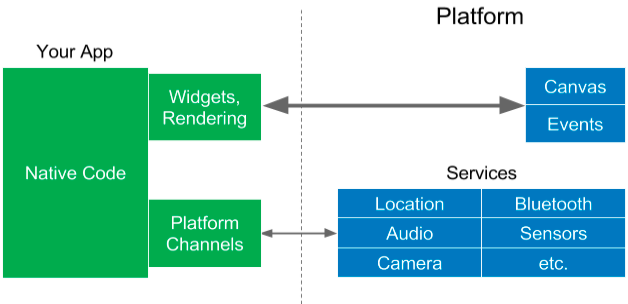
\includegraphics[width=\figureWidthModifier\linewidth]{img/stand-van-zaken/flutter-app-architecture.png}
    \caption{De architectuur van een Flutter applicatie \autocite{Leler2017}}
    \label{fig:flutter-app-architecture}
\end{figure}

Andere cross-platform frameworks zoals React Native, maken gebruik van een vertaler. In het geval van React Native is dit de JavaScript Bridge. De geschreven JavaScript code wordt door de JavaScript Bridge omgezet om de native platformen te kunnen aanspreken, zoals te zien op figuur \ref{fig:react-native-app-architecture}  \autocite{Kuitunen2019}

\begin{figure}[H]
    \centering
    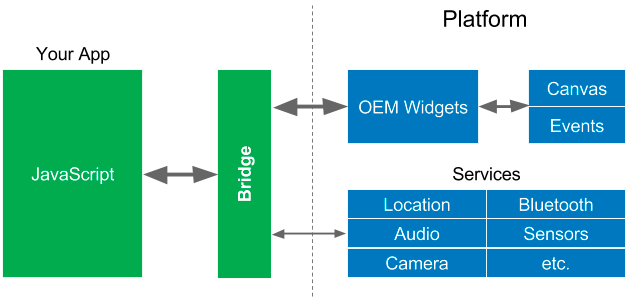
\includegraphics[width=\figureWidthModifier\linewidth]{img/stand-van-zaken/react-native-app-architecture.png}
    \caption{De architectuur van een React Native applicatie \autocite{Leler2017}}
    \label{fig:react-native-app-architecture}
\end{figure}

\subsection{Flutter Web}
Flutter heeft hoofdzakelijk als platform mobiele apparaten, maar is zeker niet beperkt tot het maken van mobiele apps. Zo is Flutter Web in Flutter versie 1.12.13 beschikbaar in beta. Aangezien Flutter web zich nog in beta bevindt, wordt er aangeraden om Flutter web nog niet te gebruiken in productie. De werking van Flutter Web wordt in deze sectie verder besproken.
\newline
Opnieuw maakt de programmeertaal Dart het mogelijk om de Flutter code te compileren naar HTML, CSS en JavaScript.

Voor Flutter Web was het nodig dat de \verb|dart:ui| opnieuw geïmplementeerd werd. De \verb|dart:ui| library bestaat uit de laagst mogelijke services die Flutter gebruikt om toepassingen op te bouwen. Bijvoorbeeld klassen voor het aansturen van de invoer en grafische tekst. Hier werd de code die beroep deed op de Skia Engine, herschreven naar doelgroepen als DOM en Canvas. De Skia Graphics Engine is een open-source grafische bibliotheek geschreven in C++. De \verb|dart:ui| library zorgt ervoor dat de Dart code gecompileerd wordt naar JavaScript en dus geschikt is voor webapplicaties. Indien een widget niet omgezet kan worden in JavaScript, HTML en CSS, wordt het widget geschilderd op een canvas.
\newline
Met Flutter Web is het Flutter framework opnieuw een stap dichter naar een volledig cross-platform ontiwkkelingsomgeving.
Deze structuur wordt weergegeven in figuur \ref{fig:flutter-web-architecture}
\begin{figure}[H]
    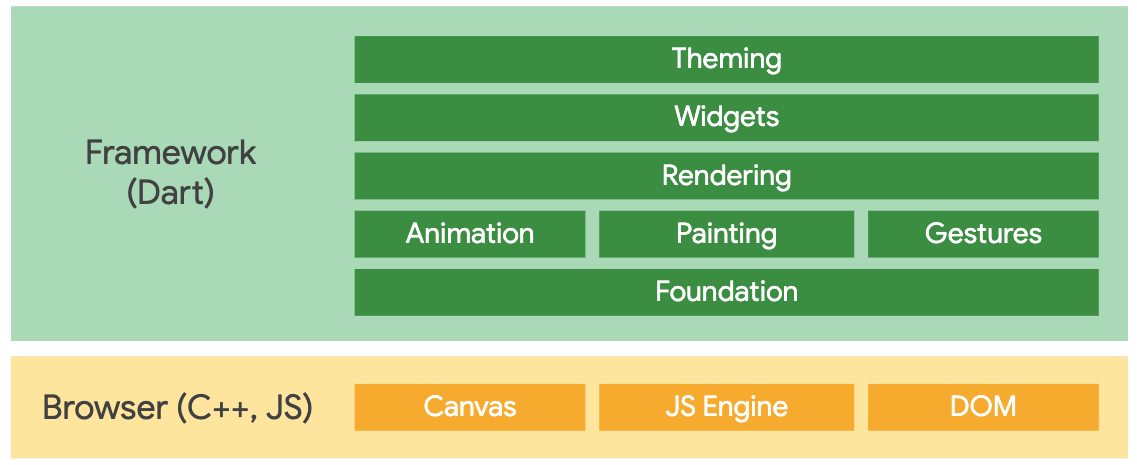
\includegraphics[width=\linewidth]{img/stand-van-zaken/flutter-web-architecture.png}
    \caption{De architectuur van Flutter Web \autocite{Flutter2019}}
    \label{fig:flutter-web-architecture}
\end{figure}


\subsection{Dart}
\label{ch:dart}
De taal die Flutter gebruikt is Dart. De populariteit van deze taal is de laatste tijd gestegen, mede dankzij de populariteit van Flutter. Met een groei van 532\% afgelopen jaar, kan Dart bekroond worden als de snelst groeiende taal \autocite{Chan2019}. 
Dit gedeelte is voornamelijk gebaseerd op een artikel van een Senior Software Engineer bij Google, Wm Leler \autocite{Leler2017a}.

De syntax van Dart is gelijkaardig aan die van Java, C\# en Javascript.
Een belangrijke troef van Dart is dat het zowel Ahead Of Time (AOT) als Just In Time (JIT) gecompileerd kan worden. Het feit dat Dart AOT gecompileerd kan worden heeft als gevolg dat een Flutter app in productie gebruik maakt van native prestaties. Dit zorgt voor een snelle en performante applicatie in productie.
De JIT compilatie lost de verwachtingen van elke ontwikkelaar in. De JIT zorgt ervoor dat wijzigingen tijdens het ontwikkelen van de applicatie quasi direct zichtbaar zijn op het apparaat. De JIT ondersteuning in Dart maakt het mogelijk dat Flutter over Hot Reloading beschikt. \autocite{Leler2017a}
\newline
Op dit moment is de laatste stabiele versie van Dart 2.7.0. Met nieuwe toevoegingen in versie 2.3.0 zoals de spread operator (...) wordt Dart frequent bijgewerkt met nieuwe features. De verwachtingen van de ontwikkelaars worden ingelost door periodiek feedback te vragen aan de community \autocite{Thomsen2019}.

\section{State en State Management}
In deze sectie wordt het concept state en de bijhorende State Management uitvoerig besproken. Dit hoofdstuk is losstaand van Flutter, maar gaat dieper in op de begrippen state en State Management. Dit onderdeel is een aanleiding naar de volgende sectie State Management in Flutter. Het is nodig om deze sectie te begrijpen om verder te gaan met dit onderzoek.

\subsection{State}
\label{ch:state}
De state van een applicatie is alles dat bijgehouden wordt in het geheugen terwijl de applicatie draait \autocite{DeConinck2019}.
Een simpel voorbeeld van state is het volgende: één invoerveld voor voornaam, één invoerveld voor achternaam en één knop die niet klikbaar is, de state van deze knop kan beschouwd worden als een variabele \textit{klikbaar = onwaar}. Op dit moment is de knop niet klikbaar. Indien de invoervelden een geldige invoer ontvangen, wordt de state van de knop bijgewerkt: \textit{klikaar = waar}. Dit resulteert in een klikbare knop. De state van de knop is afhankelijk van de state van de invoervelden. Dit is een relatief simpel voorbeeld, maar wanneer een applicatie groeit wordt dit een zeer complex probleem. Bijvoorbeeld wanneer een state van een bericht afhankelijk is van een factor op een andere pagina. De state zal op verschillende schermen gedeeld moeten worden.
In de breedst mogelijke zin is de state van een applicatie alles wat in het geheugen bestaat wanneer de app wordt uitgevoerd. 

\subsection{Het begrip State Management}
De manier waarop de state van een applicatie wordt benaderd, wordt State Management genoemd. Er zijn reeds tal van State Management libraries, zoals Redux en MobX die deze benadering vereenvoudigen. Deze benaderingen worden verder besproken in sectie \ref{ch:redux} en \ref{ch:mobx}. De bedoeling van een benadering van State Management is om de state op een overzichtelijke manier te beheren en makkelijk uit te breiden.

\section{State Management in Flutter}
De vorige secties in verband met state en State Management zijn losstaand van Flutter. In deze sectie wordt bekeken hoe de state specifiek in een Flutter applicatie kan benaderd worden.

\subsection{Ephemeral State en App State}
De Flutter documentatie definieert twee soorten states: Ephemeral State (lokaal) en App State (globaal).
Ephemeral State is de lokale state, ook wel de UI state genoemd. Deze state wordt beheerd door één enkele widget, bijvoorbeeld de geselecteerde index bij een tabbalk. Andere widgets zullen zelden dit soort state van buitenaf nodig hebben. Bij Ephemeral State is het niet nodig om een bepaalde benadering van State Management toe te passen op een widget. In dit geval kan de Stateful widget zijn state aanpassen door zijn \verb|setState()| functie aan te roepen.
Om terug het voorbeeld van het invoerveld te hernemen: er wordt geluisterd wanneer er een karakter wordt getypt in het veld. Vervolgens wordt de state van het invoerveld bijgewerkt en hierna wordt \verb|setState()| opgeroepen zodat het widget opnieuw wordt opgebouwd met de bijgewerkte waarde.
\newline \newline
De andere soort state volgens de Flutter documentatie \autocite{Developers2019} is App State, ook wel shared state genoemd. Deze soort state wordt door verschillende widgets van de applicatie gedeeld.
Een voorbeeld van dit soort state: een lijst van nieuws artikels, die respectievelijk gemarkeerd kunnen worden als gelezen en niet-gelezen. Wanneer een artikel gemarkeerd is als gelezen dan moet deze verwijderd worden uit de lijst. 
\newline

Over het algemeen is er geen duidelijke regel wanneer Ephemeral State of App State gebruikt moet worden. Dit is volledig afhankelijk van de complexiteit van de applicatie en de persoonlijke voorkeur van de ontwikkelaar.
Wanneer een applicatie nood heeft aan de nodige complexiteit wordt er aangeraden om over te schakelen naar App State, zie figuur \ref{fig:ephemeral-vs-app-state-flutter}. Theoretisch is het mogelijk om een volledige applicatie te ontwikkelen met State en setState(), maar dit wordt afgeraden \autocite{Developers2019}.
\begin{figure}[H]
    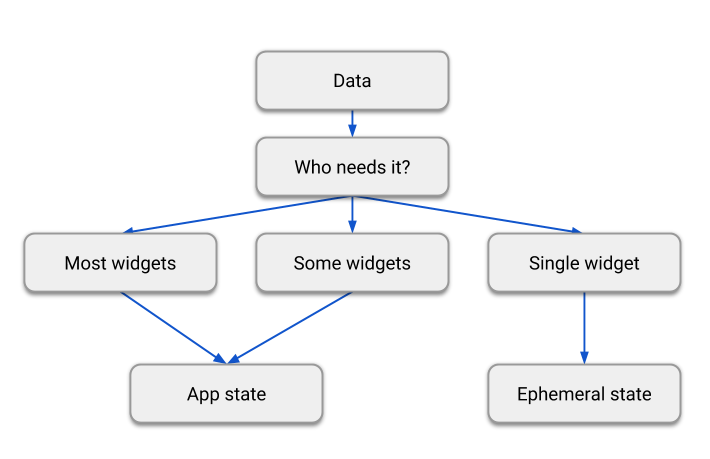
\includegraphics[width=\linewidth]{img/stand-van-zaken/ephemeral-vs-app-state-flutter.png}
    \caption{Ephemeral- vs App state in Flutter \autocite{Developers2019}}
    \label{fig:ephemeral-vs-app-state-flutter}
\end{figure}

Dit resulteert in het ontstaan van verschillende State Management benaderingen. Tal van benaderingen van State Management worden beschikbaar gesteld door middel van libraries. Deze State Mangement libraries zorgen dat het beheren van state in een applicatie versimpeld wordt.
Het doel van een State Management is om het leven van de ontwikkelaar eenvoudiger te
maken door state makkelijker beheersbaar te maken. Verder wordt de UI gescheiden van
de business logica, waardoor deze logica makkelijker getest kan worden.

In volgende sectie worden de verschillende benaderingen van State Management in Flutter besproken.
De verschillende benaderingen die besproken worden zijn: 
\begin{itemize}
    \item ScopedModel
    \item Provider
    \item BLoC met RxDart
    \item Redux
    \item MobX
\end{itemize}

\subsection{ScopedModel}
Wanneer er nood is aan een relatief simpele benadering van State Management in een Flutter applicatie is ScopedModel een geschikte kandidaat \autocite{Boelens2019}. ScopedModel geeft een Model door naar onderliggende widgets, \textit{van vader naar kinderen}. ScopedModel is opgebouwd rond drie belangrijke concepten, een Model, een ScopedModel en een ScopedModelDescendant die te zien zijn op figuur \ref{fig:scopedmodel}. 

\begin{figure}[H]
    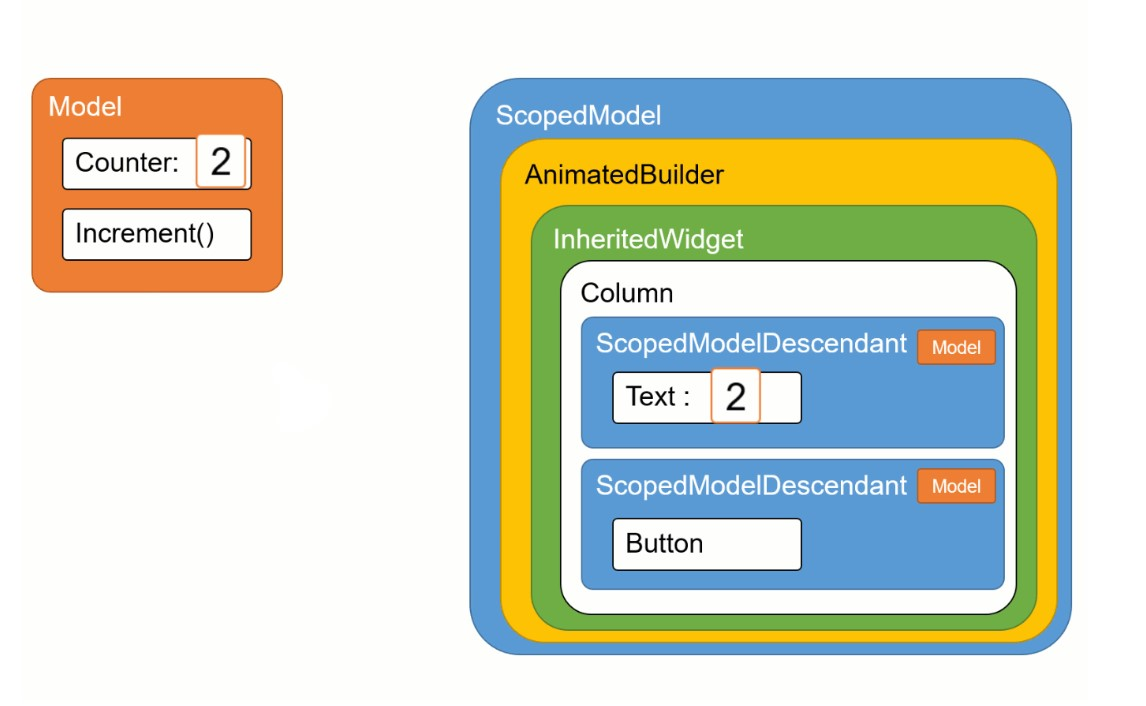
\includegraphics[width=\linewidth]{img/stand-van-zaken/scopedmodel.jpg}
    \caption{De drie concepten bij ScopedModel \autocite{Boelens2019}}
    \label{fig:scopedmodel}
\end{figure}
Als eerste wordt een klasse gedefinieerd die de 
data en business logica zal bijhouden. Deze klasse heeft als kenmerk dat er geluisterd kan worden naar deze klasse. Als er in de Model klasse een wijziging aangebracht wordt laat de klasse de wijziging aan zijn kinderen weten via \verb|notifyListeners()|.
\newline
De ScopedModel widget maakt het mogelijk om een Model mee te geven, dit zorgt ervoor dat al de kinderen van deze ScopedModel toegang hebben tot het meegegeven Model. Een kind van een ScopedModel kan het Model oproepen met \verb|ScopedModel.of<Model>(context)|.

Als laatste gebruikt ScopedModel een ScopedModelDescendant, dit is een speciale widget. Deze widget reageert automatisch op wijzigingen in het Model. Als \verb|notifyListeners()| wordt opgeroepen wordt de \verb|ScopedModelDescendant| widget opnieuw gebouwd.
ScopedModelDescendant heeft een verplichte \verb|builder| functie. Het type van Model waar de widget naar luistert wordt gedefinieerd tussen \verb|< >|
\begin{minted}{dart}
ScopedModelDescendant<CounterModel>(
    builder: (context, child, model) {
        return Text(model.counter);
    },
);
\end{minted}
Hier wordt geluisterd naar een wijziging in een \verb|CounterModel|. Wanneer deze wijzigt, met andere woorden \verb|notifyListeners()| wordt opgeroepen in het model, wordt de \verb|builder| functie aangeroepen. De waarde van de counter wordt op het scherm getoond. Nu is het mogelijk om op een ander scherm de counter te verhogen en wordt de tekst automatisch opnieuw opgebouwd. Er kan ook gebruik gemaakt worden van \verb|ScopedModel.of<CounterModel>(context)| om het model in eender welke widget op te roepen. 

Indien nood is aan meerdere modellen, kunnen de ScopedModelDescendant widgets genest worden of opnieuw via de static methode \verb|ScopedModel.of| opgeroepen worden.

\subsection{Provider}
\subsubsection{Principes}
Een nieuwkomer in het Flutter framework wordt aangeraden om de Provider benadering te hanteren. Provider zorgt voor een snelle benadering van State Management zonder al te veel complexiteit. Provider is beschikbaar in Flutter door middel van de Provider package. Provider biedt een oplossing voor State Management en Dependency Injection.
De Provider package maakt het mogelijk om data beschikbaar te maken voor widgets die het nodig hebben. Op voorwaarde dat de Provider widget als voorouder wordt geplaatst in de widget tree.

De volgende code is gegeven:
\begin{minted}{dart}
Provider<CounterModel>(
    builder: (BuildContext context) => CounterModel(),
    dispose: (BuildContext context, CounterModel counterModel) {
        counterModel.dispose(),
    },
    child: Container(),
);
\end{minted}

Hier wordt een CounterModel eenmalig aangemaakt. Vervolgens wordt met de \verb|dispose()| methode meegegeven wat er moet gebeuren als het Provider widget wordt verwijderd uit de widget tree. Nu is het mogelijk om in de kinderen van de Provider widget het CounterModel op te vragen via \verb|final counterModel = Provider.of<CounterModel>(context)|.
Bijvoorbeeld in de Container die wordt meegegeven aan het \verb|child| property.

De functie \verb|Provider.of<T>(context, listen: false)| heeft zoals gegeven een \verb|listen| optie. Als \verb|false| wordt meegegeven wordt de widget niet herbouwd bij een wijziging. Bij sommige omstandigheden kan dit van toepassing zijn zodat onnodige rebuilds vermeden worden. Aangezien de Provider widget de totale controle heeft over het moment waarop de waarde wordt opgevraagd is er een zekerheid dat de waarde niet tweemaal wordt opgevraagd. Met andere woorden de waarde wordt niet tweemaal geïnstantieerd.

\subsubsection{Werking}
De werking van de Provider package beperkt zich niet alleen tot het voorzien (provide) van een waarde, maar heeft zoals eerder vermeld, ook een meldfunctionaliteit (notify).
In de documentatie van de package zijn tal van Provider variaties beschikbaar: \verb|ListenableProvider|, \verb|ChangeNotifierProvider|, \verb|ChangeNotifierProxyProvider|, \verb|ValueListenableProvider|, \verb|StreamProvider| en \verb|FutureProvider|. Als laatste is, zoals reeds vermeld, een \verb|Consumer| widget beschikbaar.
De \verb|ListenableProvider| is een specifieke implementatie voor het \verb|Listenable| object. De \verb|ListenableProvider| luistert naar data en vraagt aan de afhankelijke widgets om opnieuw te renderen wanneer de listener wordt opgeroepen. In de praktijk wordt de \verb|ListenableProvider| niet direct gebruikt, maar wel indirect. De \verb|ChangeNotifierProvider| is een specificatie van de \verb|ListenableProvider| voor \verb|ChangeNotifier|. Hier wordt de \verb|ChangeNotfier.dispose| automatisch opgeroepen wanneer nodig.

Recentelijk is de \verb|MultiProvider| toegevoegd. Deze widget biedt een oplossing tegen het nesten van Provider widgets. Stel er is nood aan twee modellen doorheen een applicatie. Het eerste model wordt meegegeven aan de Provider widget. Het tweede model wordt opnieuw meegegeven aan een Provider widget. Dit resulteert in volgende code:
 \begin{minted}{dart}
 Provider<CounterModel>(
    builder: (BuildContext context) => CounterModal(),
    dispose: (BuildContext context, CounterModel counterModel) {
        counterModel.dispose(),
    },
    child: Provider<PreferenceModel>(
        builder: (BuildContext context) => PreferenceModel(),
        dispose: (BuildContext context, PreferenceModel preferenceModel) {
            preferenceModel.dispose(),
        },
    ),
);
\end{minted}
Dit resulteert in het nesten van Provider widgets, dit probleem wordt opgelost door de \verb|MultiProvider|. Volgende code is idem aan bovenstaande, maar is overzichtelijker en stimuleert de leesbaarheid van de code.
 \begin{minted}{dart}
MultiProvider(
    providers: [
        Provider<CounterModel>(
            builder: (BuildContext context) => CounterModel(),
            dispose: (BuildContext context, CounterModel counterModel) {
                counterModel.dispose(),
            },
        ),
        Provider<PreferenceModel>(
            builder: (BuildContext context) => PreferenceModel(),
            dispose: (BuildContext context, PreferenceModel preferenceModel) {
                preferenceModel.dispose(),
            },
        ),
    ],
    child: Container(),
);

\end{minted}

De Provider package biedt twee manieren aan om op de hoogte te worden gebracht.
\newline
De eerste manier is via de static methode \verb|Provider.of(context)| met een optionele \verb|listen| property, standaard op \verb|true|.
Wanneer een widget zichzelf registreert als een dependency van de Provider InheritedWidget, zal het telkens opnieuw opgebouwd worden wanneer de data wijzigt. Een InheritedWidget is een klasse voor widgets die informatie efficiënt door de boom heen wil verspreiden.
 Meer bepaald wanneer \verb|notifyListeners()| wordt opgeroepen. Of wanneer een \verb|StreamProvider| zijn stream nieuwe data uitzendt of wanneer een \verb|FutureProvider| zijn future is voltooid. Een Future in Dart wordt gebruikt om een potentiële waarde of fout weer te geven die ergens in de toekomst beschikbaar zal zijn, met andere woorden een asynchrone operatie. Een future is te vergelijkbaar met een Promise in JavaScript.

De tweede manier is om gebruik te maken van de \verb|Consumer| widget. Deze widget is een hulp widget die in de achtergrond de \verb|Provider.of(context)| gebruikt. De werking van de \verb|Consumer| is gelijkaardig aan die van de bovenstaande. 

De \verb|Provider| package is gelijkaardig aan de \verb|ScopedModel| benadering. Waar \verb|Provider| een volledige oplossing biedt voor dependency injection, probeert \verb|ScopedModel| zich op te stellen als een architecturale oplossing.

\subsection{BLoC met RxDart}
\subsubsection{Business Logic Component}
Het BLoC patroon dat staat als afkorting voor Business Logic Component. Het BLoC werd oorspronkelijk aangeboden als oplossing voor het delen van dezelfde business logica tussen Flutter en AngularDart. AngularDart is een open-source project gebouwd bovenop het Dart Web Platform, het wordt veelal gebruikt voor het ontwikkelen van webapplicaties in Dart. Hedendaags wordt BLoC door Google aangeraden als een superieure State Management techniek. Het BLoC pattern maakt gebruik van Streams die beschikbaar zijn in Dart, maar vaak wordt beroep gedaan op een gebruiksvriendelijkere library namelijk ReactiveX, zie \ref{ch:reactivex}. De ReactiveX library is een laag bovenop de Streams.
\newline \newline
De ReactiveX (rX) library is in Dart beschikbaar onder de naam RxDart.

\subsubsection{Streams}
Om het BLoC patroon volledig te begrijpen moet het concept Streams uitgelegd worden.
Een stream kan gevisualiseerd worden als een pipe met twee uiteinden, waarvan slechts
één uiteinde gebruikt kan worden om iets in de pipe te plaatsen en het andere dient als de uitgang. Wanneer data in de pipe
geplaatst wordt, stroomt het door de pipe naar het andere uiteinde. \autocite{Boelens2018}

\begin{figure}[H]
    \centering
    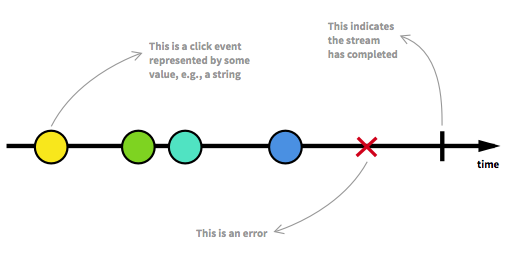
\includegraphics[width=\figureWidthModifier\linewidth]{img/stand-van-zaken/stream-pipeline.png}
    \caption{Voorbeeld van een Stream pipeline \autocite{Staltz2019}} 
    \label{fig:stream-pipeline}
\end{figure}

In Flutter kan het concept van Streams gemakkelijk gebruikt worden. De effectieve pipe wordt voorgesteld als een Stream. Deze \verb|Stream| klasse op zich maakt het niet mogelijk om deze pipe te beheren.
Daarvoor wordt een \verb|StreamController| gebruikt. Om toegang te krijgen tot de invoer van een pipe, wordt beroep gedaan op een \verb|StreamSink|. Deze wordt door de \verb|StreamController| beschikbaar gesteld via de \verb|sink| property.

Zowel primitieve data types als objecten en errors kunnen voorgesteld worden als een stream. Een stream heeft geen beperkingen op vlak van soorten data types.

Om wijzigingen van een stream in acht te nemen kan er geluisterd worden naar een stream, dit resulteert in een \verb|StreamSubscription|. Deze \verb|StreamSubscription| is beschikbaar via de \verb|stream| property van de StreamController. Deze geeft meldingen wanneer er wijzigingen gebeuren in de stream, bijvoorbeeld wanneer een nieuwe waarde wordt toegevoegd op deze stream.

Met andere woorden heeft een pipe één toegang, de sink en één uitgang, de stream.

Als er minstens één actieve luisteraar van een stream is, start de stream met het genereren van events die de \verb|StreamSubscription| verwittigt wanneer een wijziging zich voordoet. Deze events worden opgeroepen bij volgende scenario's: er is een error in de stream, de stream wordt afgesloten of er is nieuwe data in de stream.

De \verb|StreamTransformer| zorgt ervoor dat de data in de stream gemanipuleerd kan worden. Onder deze manipulaties worden volgende verstaan: filteren, hergroeperen, aanpassen, data in andere streams injecteren...
Een voorbeeld van een StreamTransformer manipulatie op een Stream:
 \begin{minted}{dart}
final streamTransformer = StreamTransformer<num, num>.fromHandlers(
    handleData: (num data, EventSink sink) {
        // De data wordt vermenigvuldigd met 2
        sink.add(data * 2);
    }, 
    handleError: (Object error, StackTrace stacktrace, EventSink sink) {
        // Voeg de error toe aan de stream via de sink
        sink.addError('Er ging iets fout: $error');
    }, 
    handleDone: (EventSink sink) => sink.close(),
);
\end{minted}

Bij streams zijn er twee soorten types: single-subscription- en broadcast streams. Bij een single-subscription stream kan er slechts één luisteraar geabonneerd zijn, zelfs wanneer de subscription geannuleerd wordt. Indien er een tweede maal geluisterd wordt naar een single-subscription stream wordt een gepaste error gegeven: \verb| Stream has already been listened to|.

Bij een broadcast stream kunnen er meerdere luisteraars zijn. Het is mogelijk om op elk moment een luisteraar aan een broadcast stream toe te voegen. De nieuwe luisteraar ontvangt de gebeurtenissen vanaf het moment dat deze naar de stream begint te luisteren.

De implementatie van de stream library wordt standaard meegeleverd in de Software Development Kit (SDK) van Flutter. Om een stream te visualiseren in een widget wordt de StreamBuilder widget gebruikt. Een StreamBuilder is geïmplementeerd als een StatefulWidget die opnieuw wordt opgebouwd wanneer nieuwe events gestreamd worden.
Een voorbeeld van zo'n StreamBuilder:
\begin{minted}{dart}
StreamBuilder<Counter>(
    stream: counterStream,
    initialData: 0,
    builder: (context, snapshot) {
        if (snapshot.hasData){
            return Text(snapshot.data);
        }
        return CircularSpinner();
    },
);
\end{minted}
De initiële data wordt ingesteld op 0 wanneer de \verb|counterStream| nog geen data bevat. Dit dat de StreamBuilder widget bij de initiële render 0 zal gebruiken als data. De \verb|builder| functie zorgt ervoor dat de StreamBuilder weet welke widget opgebouwd moet worden wanneer de \verb|StreamBuilder| nieuwe data ontvangt via de \verb|stream| property.

In volgende sectie wordt het rxDart package besproken, deze package breidt de functionaliteit van de originele Dart Streams uit om te voldoen aan de ReactiveX standaarden.

\subsubsection{ReactiveX in Dart}
\label{ch:reactivex}
De ReactiveX library is een library die de functionaliteiten van streams in een programmeertaal uitbreidt. Zo is ReactiveX beschikbaar in JavaScript onder de naam RxJS, maar relevanter voor dit onderzoek, in Dart: de RxDart library.


Zoals reeds vermeld is de RxDart package een implementatie van de ReactiveX API in Dart. Zowel Dart Streams als RxDart worden gebruikt om streams te maken en beheren, maar beide ontwikkelaars gebruiken een andere terminologie.
Een Stream in Dart wordt voorgesteld als een \verb|Observable| in RxDart. Een StreamController is een \verb|Subject| in RxDart, zie tabel \ref{table:terminologie-rxdart-dart}.

\begin{table}[H]
    \centering
    \begin{tabular}{ll}
        \textbf{Dart}    & \textbf{RxDart} \\ \hline
        Stream           & Observable      \\
        StreamController & Subject         \\
        &                
    \end{tabular}
    \caption{Verschillende stream terminologie in Dart en RxDart \autocite{Boelens2018}}
    \label{table:terminologie-rxdart-dart}
\end{table}

RxDart biedt drie variaties van de StreamController.
\newline 
De PublishSubject, geïllustreerd op figuur \ref{fig:rxdart-publishsubject}, is een normale broadcast StreamController. In dit diagram wordt enkel data van de stream gestuurd, nadat er naar de stream geluisterd (geabonneerd) wordt.
Merk op dat deze variaties een Observable terug geven in plaats van een Stream zie tabel \ref{table:terminologie-rxdart-dart}.


\begin{figure}[H]
    \centering
    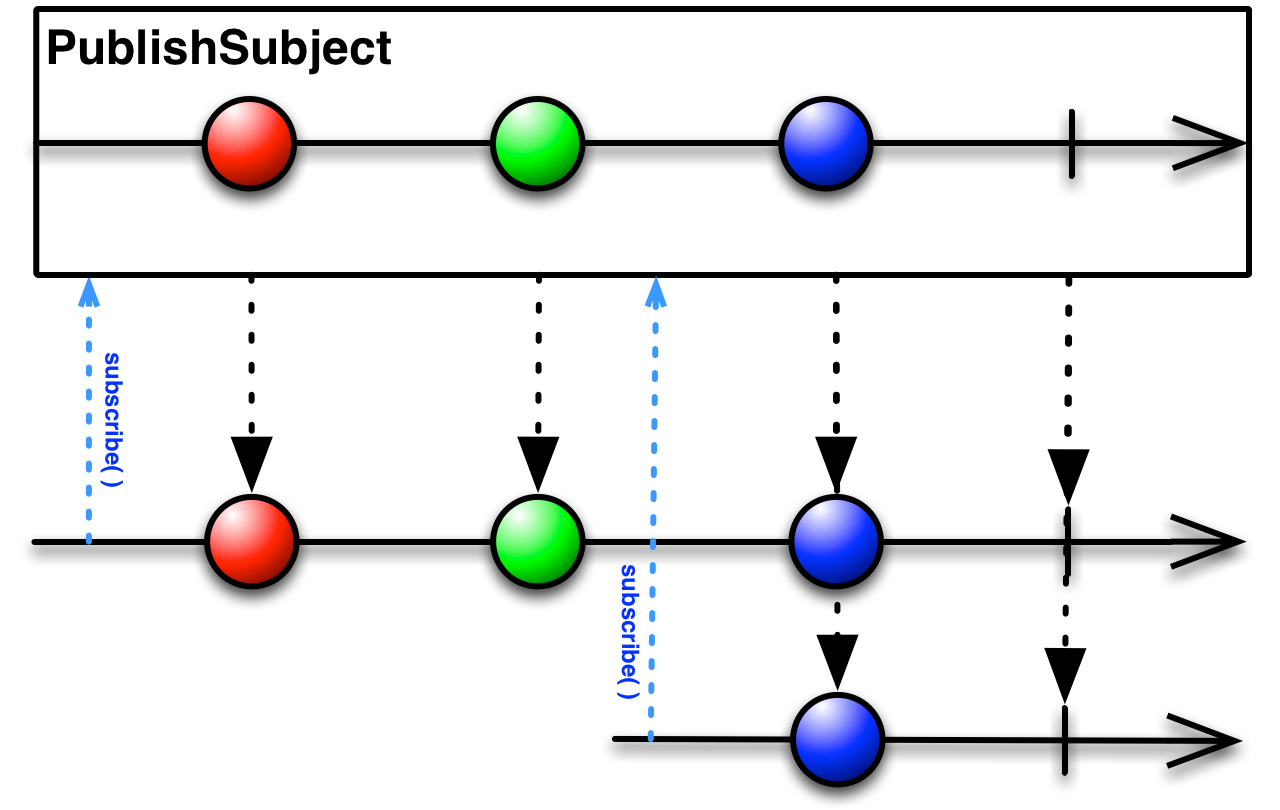
\includegraphics[width=\figureWidthModifier\linewidth]{img/stand-van-zaken/rxdart-publishsubject.png}
    \caption{Marble diagram van PublishSubject uit de ReactiveX library \autocite{Boelens2018}}
    \label{fig:rxdart-publishsubject}
\end{figure}

De tweede variatie is een BehaviorSubject, ook dit is een broadcast StreamController. Hier wordt de laatst toegevoegde data van de stream uitgezonden. Ook al was de luisteraar nog niet geabonneerd op het moment dat de laatste data werd uitgezonden. Zie figuur \ref{fig:rxdart-behaviorsubject}. 

\begin{figure}[H]
    \centering
    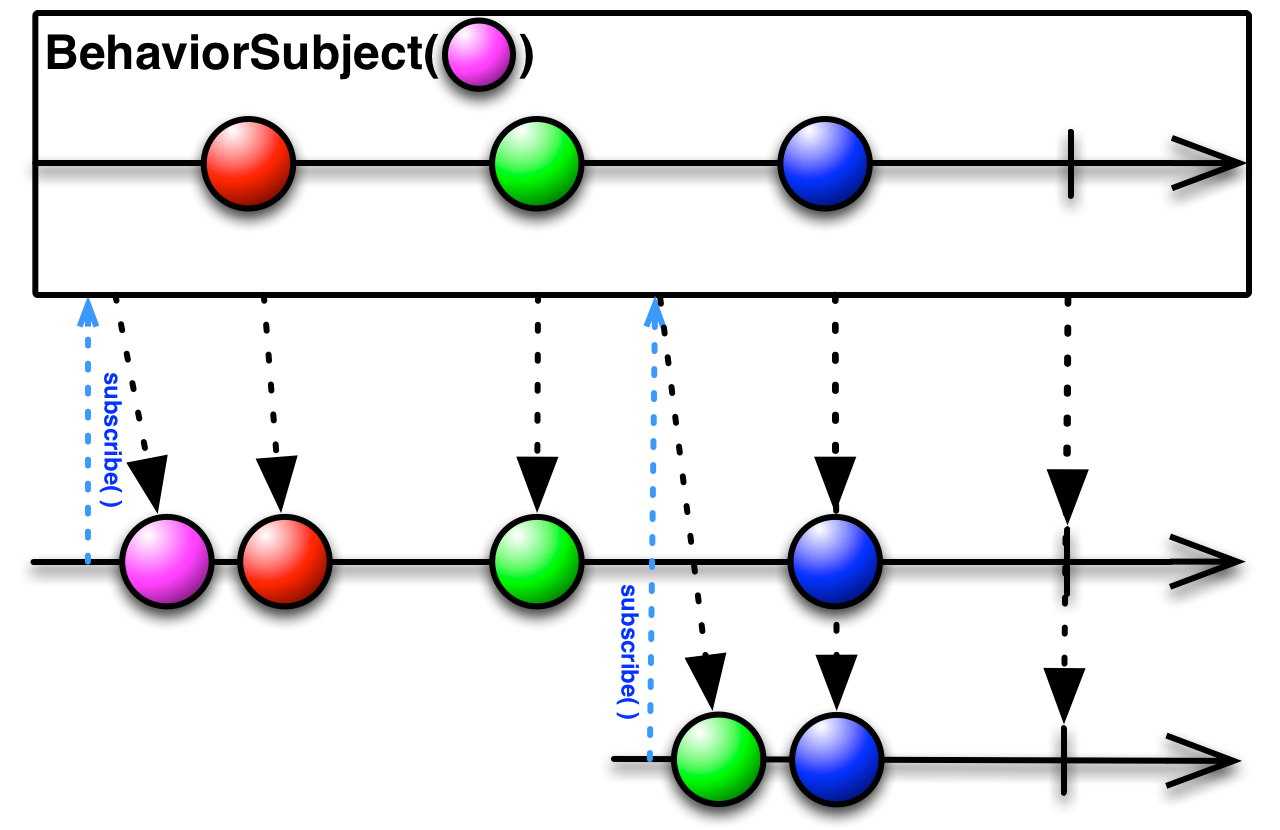
\includegraphics[width=\figureWidthModifier\linewidth]{img/stand-van-zaken/rxdart-behaviorsubject.png}
    \caption{Marble diagram van BehaviorSubject uit de ReactiveX library \autocite{Boelens2018}}
    \label{fig:rxdart-behaviorsubject}
\end{figure}

Als derde variatie is er de ReplaySubject. Dit is een broadcast StreamController die alle events uitzendt naar zijn luisteraars die reeds zijn voorgekomen sinds het begin van de stream zijn levencyclus. Zie figuur \ref{fig:rxdart-replaysubject}.

\begin{figure}[H]
    \centering
    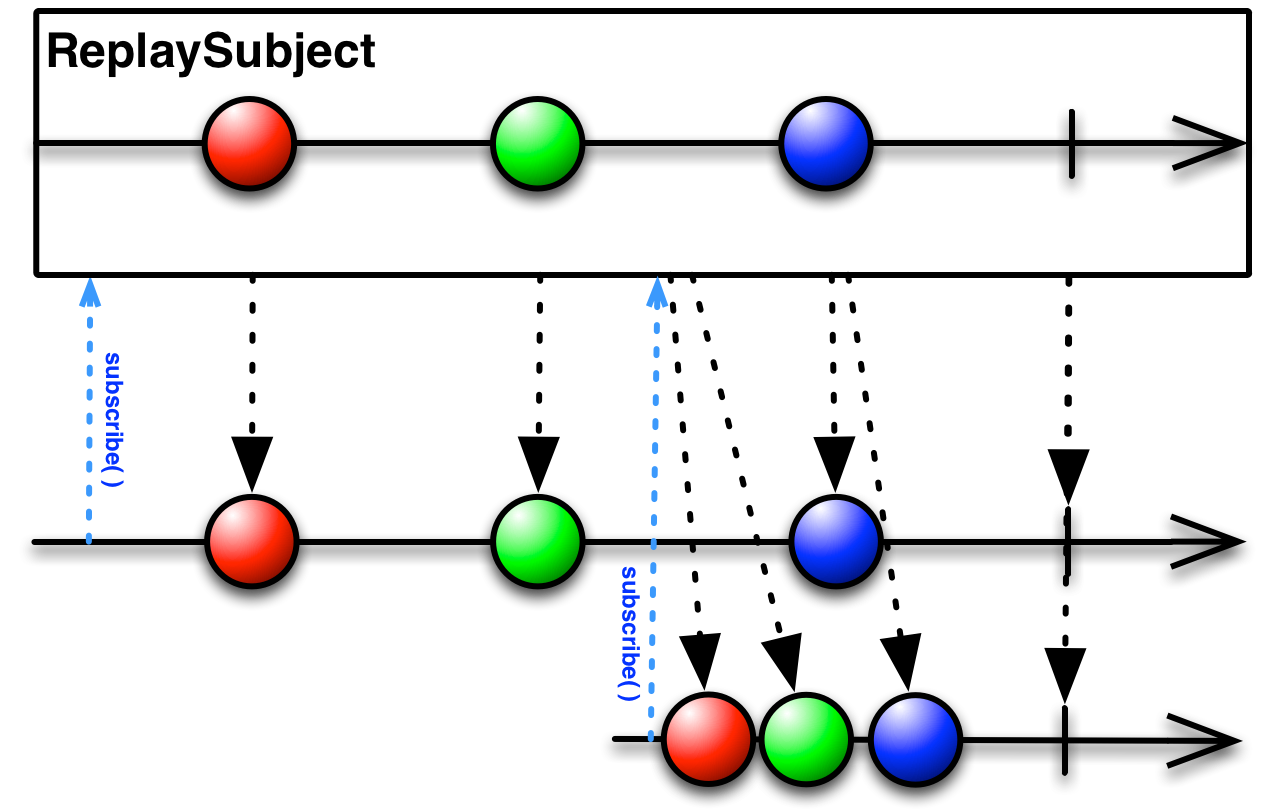
\includegraphics[width=\figureWidthModifier\linewidth]{img/stand-van-zaken/rxdart-replaysubject.png}
    \caption{Marble diagram van ReplaySubject uit de ReactiveX library\autocite{Boelens2018}}
    \label{fig:rxdart-replaysubject}
\end{figure}

\subsubsection{Het leven van het BLoC patroon}
De toepassing van het BLoC patroon is dat alle business logica zoveel mogelijk wordt losgekoppeld van de presentatie laag. Deze business logica kan opgesplitst worden in verschillende Business Logic Components (BLoCs). 
\newline
Enkele voordelen zijn: 
\begin{itemize}
    \item Er kunnen aanpassingen gedaan worden in de business logica zonder dat de presentatielaag aangepast wordt.
    \item De business logica kan makkelijk hergebruikt worden doorheen het project, zo ook voor externe projecten die beroep doen op dezelfde business logica.
    \item Het is eenvoudiger om de business logica te testen.
\end{itemize}
Zie structuur BLoC patroon op figuur \ref{fig:bloc-pattern}.

\begin{figure}[H]
    \centering
    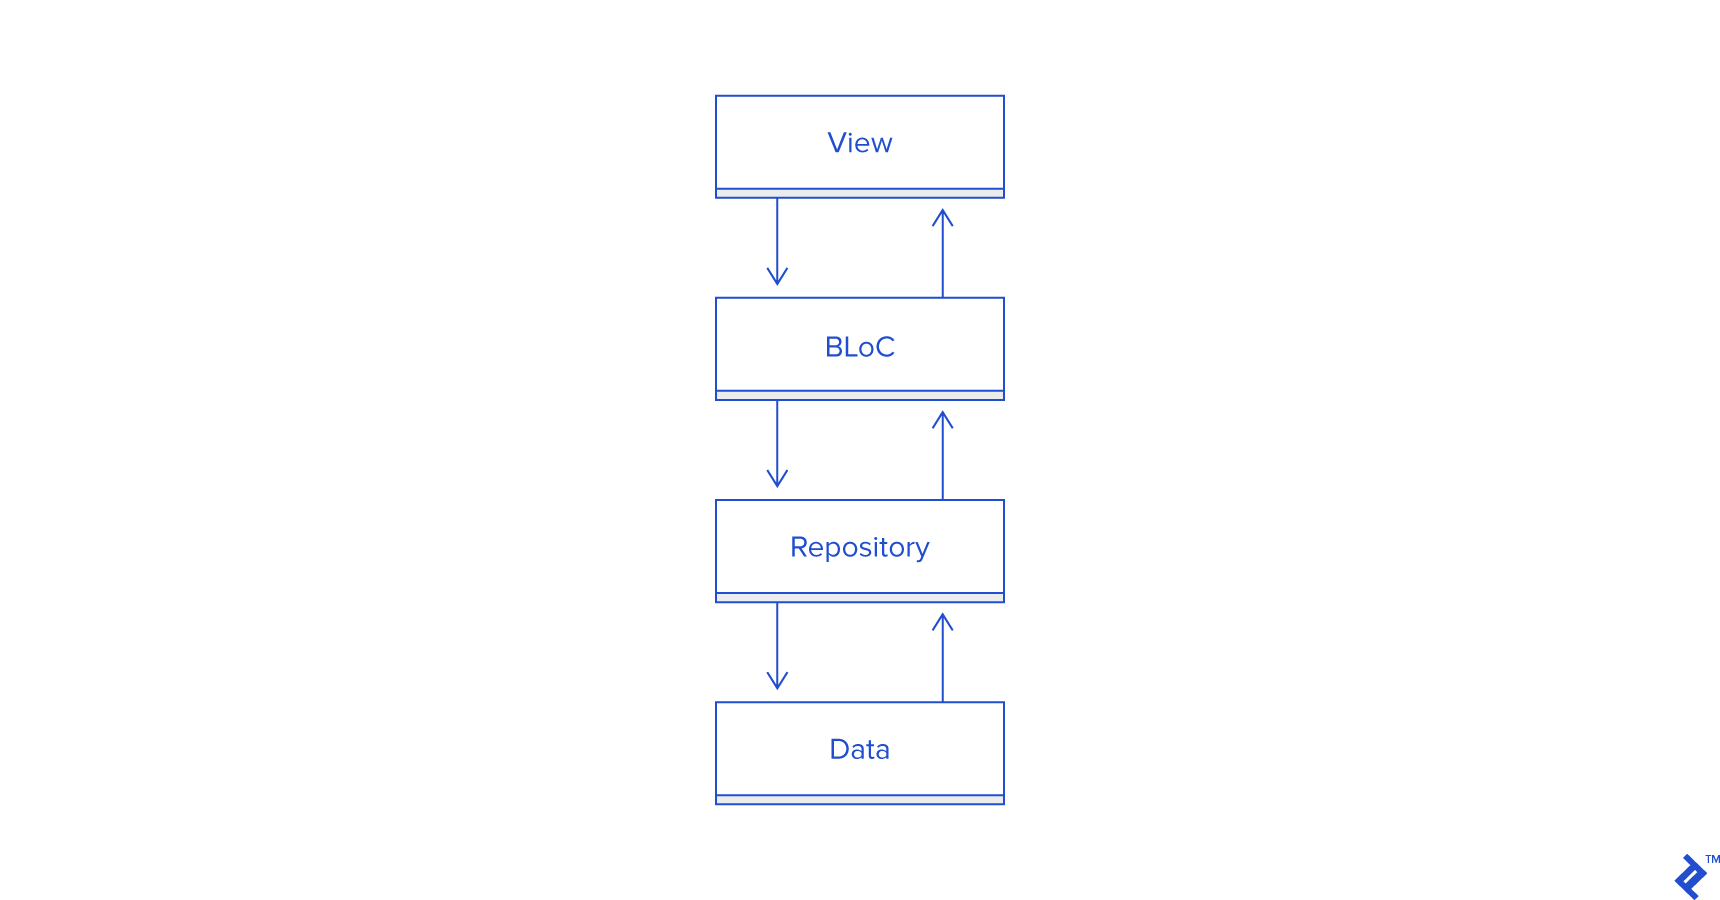
\includegraphics[width=0.9\linewidth]{img/stand-van-zaken/bloc-pattern.png}
    \caption{Concept van het BLoC patroon \autocite{Perutovic2018}}
    \label{fig:bloc-pattern}
\end{figure}

Bij het BLoC patroon zenden widgets events naar de BLoC via sinks en luisteren ze naar de streams van de BLoC.
Anders gezegd: de input van het BLoC de sink is en de output van het BLoC de stream. Een widget die luistert naar een stream wordt bijgewerkt wanneer er nieuwe data is. Bij deze benadering van State Management moet de widget in de presentatie geen kennis hebben van de business logic zoals te zien op figuur \ref{fig:bloc-pattern-streams-sinks}. \\


\begin{figure}[H]
    \centering
    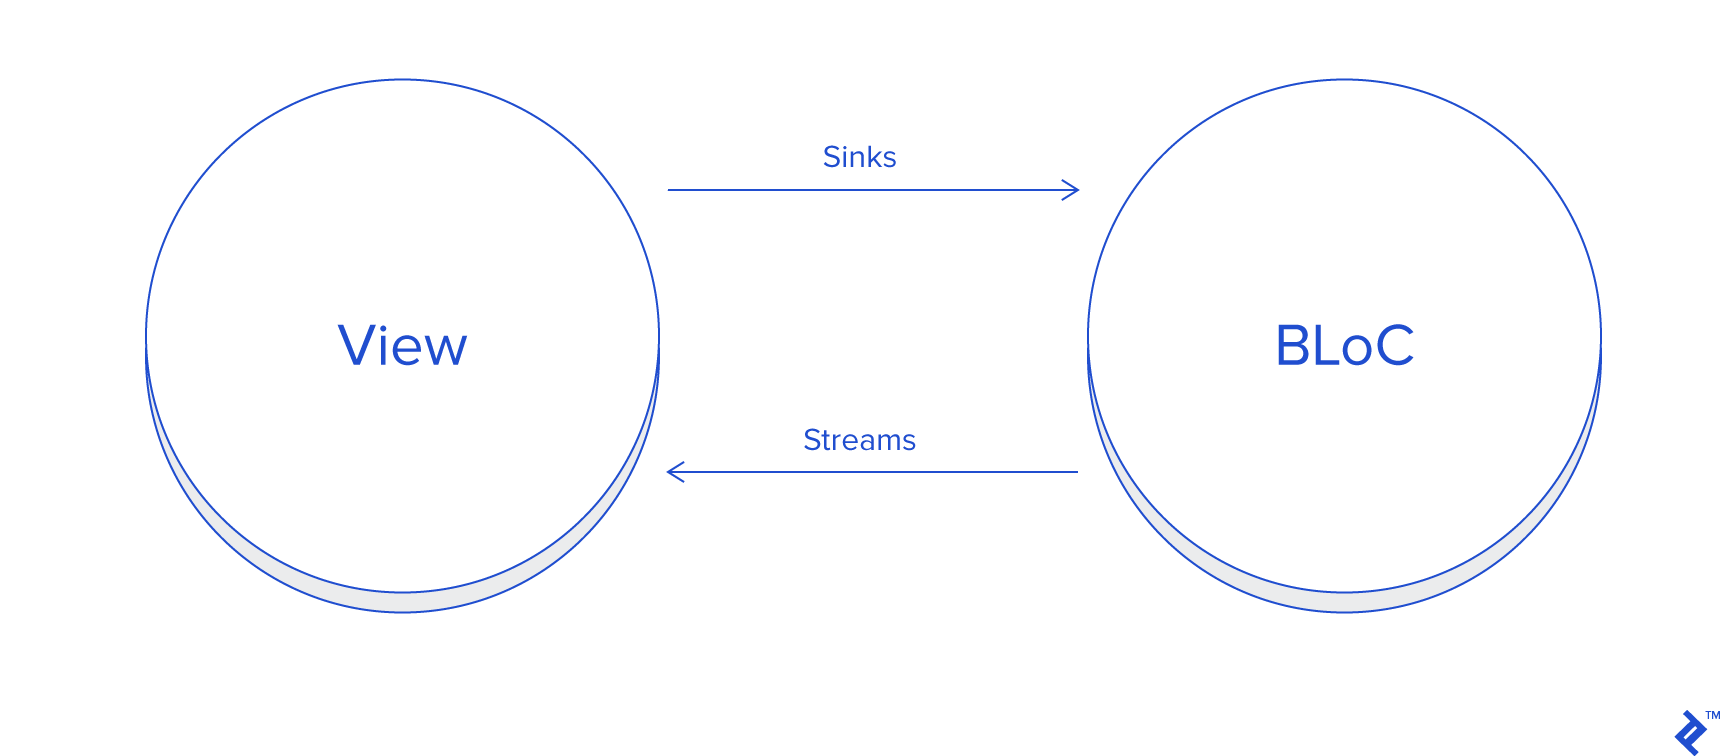
\includegraphics[width=\figureWidthModifier\linewidth]{img/stand-van-zaken/bloc-pattern-streams-sinks.png}
    \caption{Streams en Sinks tussen de presentatie en business logica \autocite{Perutovic2018}}
    \label{fig:bloc-pattern-streams-sinks}
\end{figure}

Er zijn verschillende manieren om de BLoC beschikbaar te stellen aan de widgets. 
Als eerste via een globale singleton. Dit wordt niet aangeraden aangezien er geen class destructor is in Dart, met andere woorden: mogelijkheid op memory leaks. Dart is een garbage-collected taal dit wil zeggen dat elk object, waar er geen verwijzing naar is, wordt door het runtime-systeem vrijgegeven. 
Een tweede mogelijkheid is om een lokale instantie te maken van de BLoC. Dit is een werkbare oplossing onder sommige omstandigheden. Merk hierbij op dat deze lokale instantie gemaakt wordt in een StatefulWidget, zodat de subscriptions op de streams in de \verb|dispose()| beëindigd kunnen worden.
De laatste en ook meest voorkomende manier is om de BLoC mee te geven aan een voorouder widget, die een implementatie is van een InheritedWidget of een StatefulWidget. Deze widget zorgt ervoor dat de BLoC ter beschikking gesteld wordt voor al zijn nakomelingen. Hiervoor wordt gebruikt gemaakt van een \verb|InheritedWidget|. Deze widget zorgt ervoor dat de nakomelingen in deze widget tree toegang hebben tot de BLoC.

\subsection{Redux}
\label{ch:redux}
\subsubsection{Principes}
Redux is een gekende library voor het beheren van state. De library is vooral gekend bij JavaScript ontwikkelaars en wordt vaak gebruikt in Angular of React applicaties. Angular en React zijn beiden JavaScript frameworks voor het ontwikkelen van webapplicaties. Echter is de library ook bruikbaar voor Flutter applicaties, aangezien de concepten dezelfde zijn. De package is beschikbaar in de package manager van Dart (pub.dev) onder de naam \verb|flutter_redux|.

Een toelichting over een paar begrippen die voorkomen in Redux.
Actions beschrijven alleen maar wat er gebeurd is. Elke action beschikt over een reducer, die de state aanpast.

Een Reducer is een synchrone functie die enige verwerking uitvoert op basis van de combinatie action - state. De manipulatie van de state kan leiden tot een nieuwe state in de Store. De Reducer is de enige die de state mag veranderen. Op deze manier zit de business logica alleen verwerkt in de Reducer. 

Een Middleware is een functie, meestal gericht op het uitvoeren van asynchrone taken, gebaseerd op een Action. Een Middleware maakt gebruik van State maar wijzigt deze niet. Een voorbeeld van een Middleware kan een logger functie zijn. Een ontwikkelaar kan ervoor zorgen dat elke action gelogd wordt, dit kan met behulp van een Middleware.

Redux bestaat uit een paar verschillende principes: er wordt gebruik gemaakt van een unidirectionele data flow. De store houdt maar één state bij en heeft maar één aanspreekpunt, namelijk via \verb|dispatch|. De \verb|dispatch| accepteert alleen maar \verb|actions| als argument.

Volgens de officiële documentatie van Redux \autocite{Redux2019} is het een good practice om per applicatie slechts een enkele Store te hebben. Indien het toch gewenst is om de data handling te scheiden wordt aangeraden om \verb|reducer composition| toe te passen in plaats van meerdere stores te maken.

\subsubsection{Werking}
Over het algemeen is de werking van Redux samen te vatten zoals op de figuur \ref{fig:redux-working}. Een applicatie bevat state. Deze state wordt aan een gebruiker getoond in de presentatielaag. Wanneer de presentatielaag een wijziging teweeg brengt, bijvoorbeeld door een klik op een knop, wordt een Action opgeroepen. De Action wordt ontvangen door een Reducer. Deze reducer werkt de Store bij waar de State van de applicatie wordt bijgehouden. Merk op dat deze Action door een Middleware kan passeren vooraleer deze wordt afgehandeld door een Reducer.

\begin{figure}[H]
    \centering
    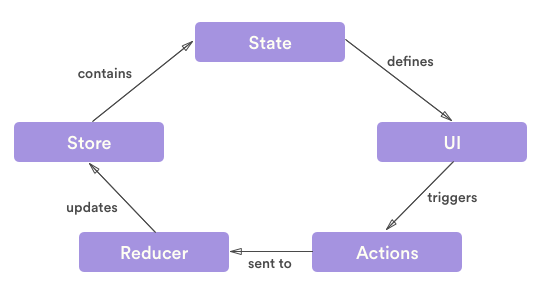
\includegraphics[width=\linewidth]{img/stand-van-zaken/redux-working.png}
    \caption{Werking van Redux \autocite{Tahir2018}}
    \label{fig:redux-working}
\end{figure}

Aangezien de manier in Redux voor vele ontwikkelaars een wijziging in de gedachtegang vereist, wordt een situatie in Redux geschetst waarbij elke stap uitvoerig wordt besproken.
Stel een applicatie toont een pagina met één knop. De applicatie bevindt zich in een initiële state. Dit wordt voorgesteld in figuur \ref{fig:redux-working-detailed-1}.

\begin{figure}[H]
    \centering
    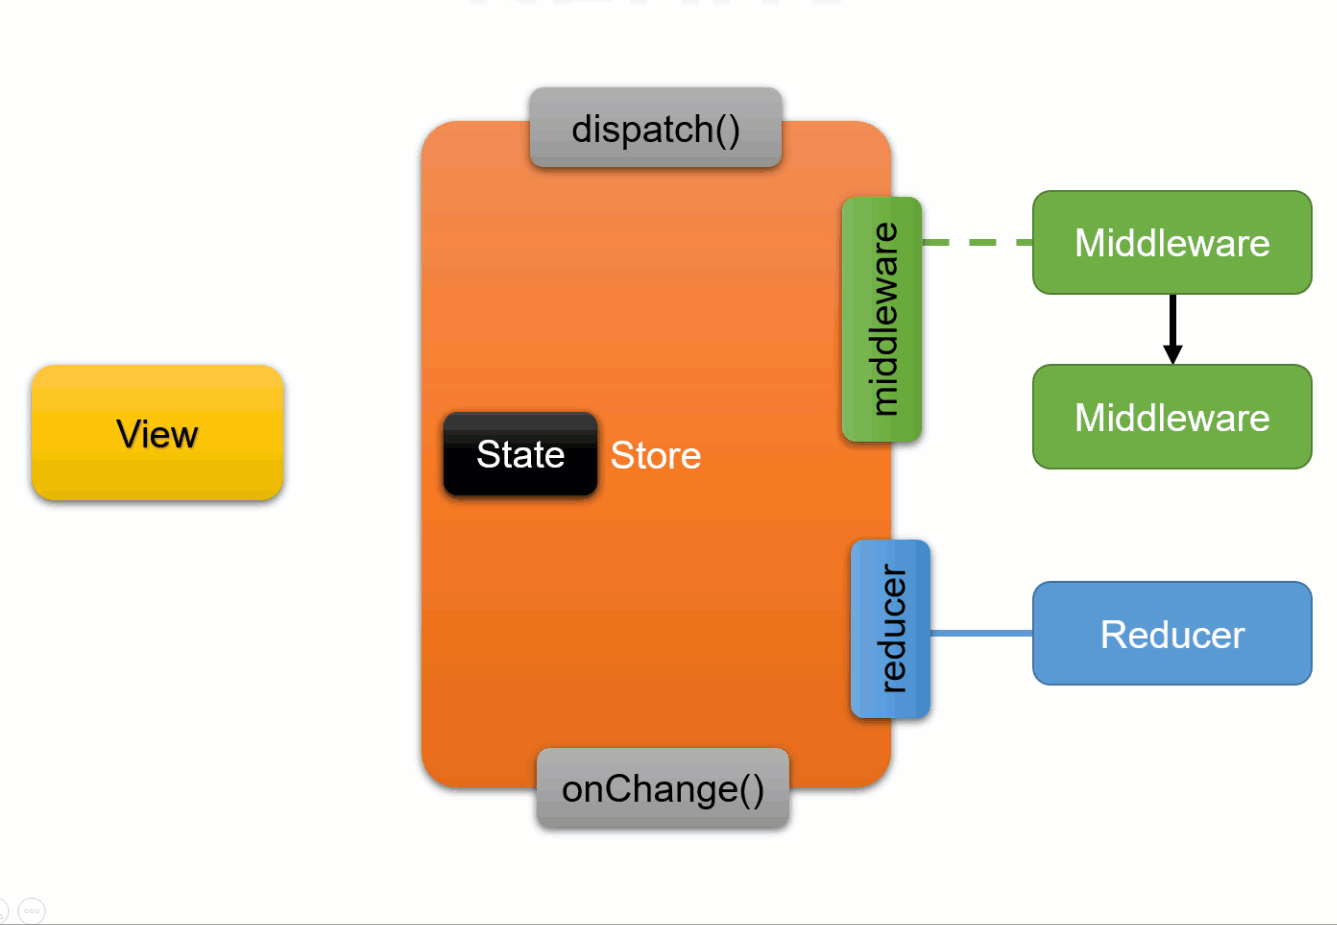
\includegraphics[width=\figureWidthModifier\linewidth]{img/stand-van-zaken/redux-working-detailed-1.png}
    \caption{Initiële situatie in een Redux State Management benadering \autocite{Boelens2019}}
    \label{fig:redux-working-detailed-1}
\end{figure}

Wanneer op een knop wordt geklikt, wordt een Action aangemaakt en uitgezonden naar de Store, dit is te zien op figuur \ref{fig:redux-working-detailed-2}. Dit uitzenden gebeurt via de \verb|store.dispatch(action)|. Indien voor de Action Middleware geconfigureerd is, wordt de Middleware sequentieel opgeroepen. Merk op dat tijdens de verwerking van deze Middleware een nieuwe Action kan verzonden worden naar de Store.

\begin{figure}[H]
    \centering
    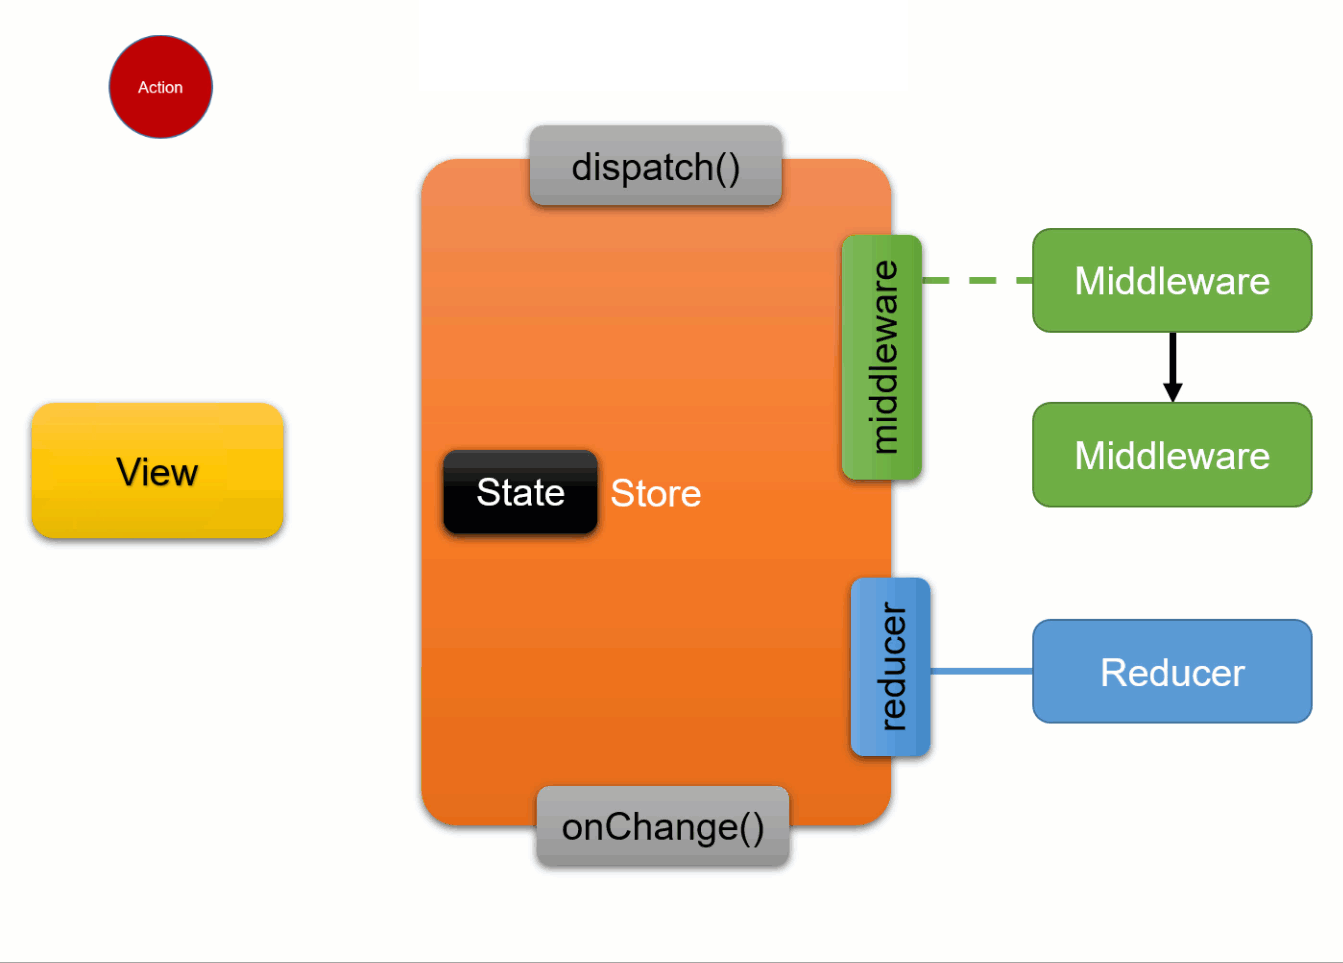
\includegraphics[width=\figureWidthModifier\linewidth]{img/stand-van-zaken/redux-working-detailed-2.png}
    \caption{een Action wordt gemaakt en verzonden naar de Store \autocite{Boelens2019}}
    \label{fig:redux-working-detailed-2}
\end{figure}

Vervolgens worden de Action en de nieuwe State doorgestuurd naar de Reducer, te zien op figuur \ref{fig:redux-working-detailed-3}. De Reducer zal zoals reeds gezegd de State aanpassen, enkel en alleen de Reducer heeft de mogelijkheid om de State te muteren. 
De Store zorgt ervoor dat alle luisteraars worden geïnformeerd wanneer de State is aangepast. De view zal op zijn beurt worden aangepast op basis van de nieuwe State, zie figuur \ref{fig:redux-working-detailed-4}.

\begin{figure}[H]
    \centering
    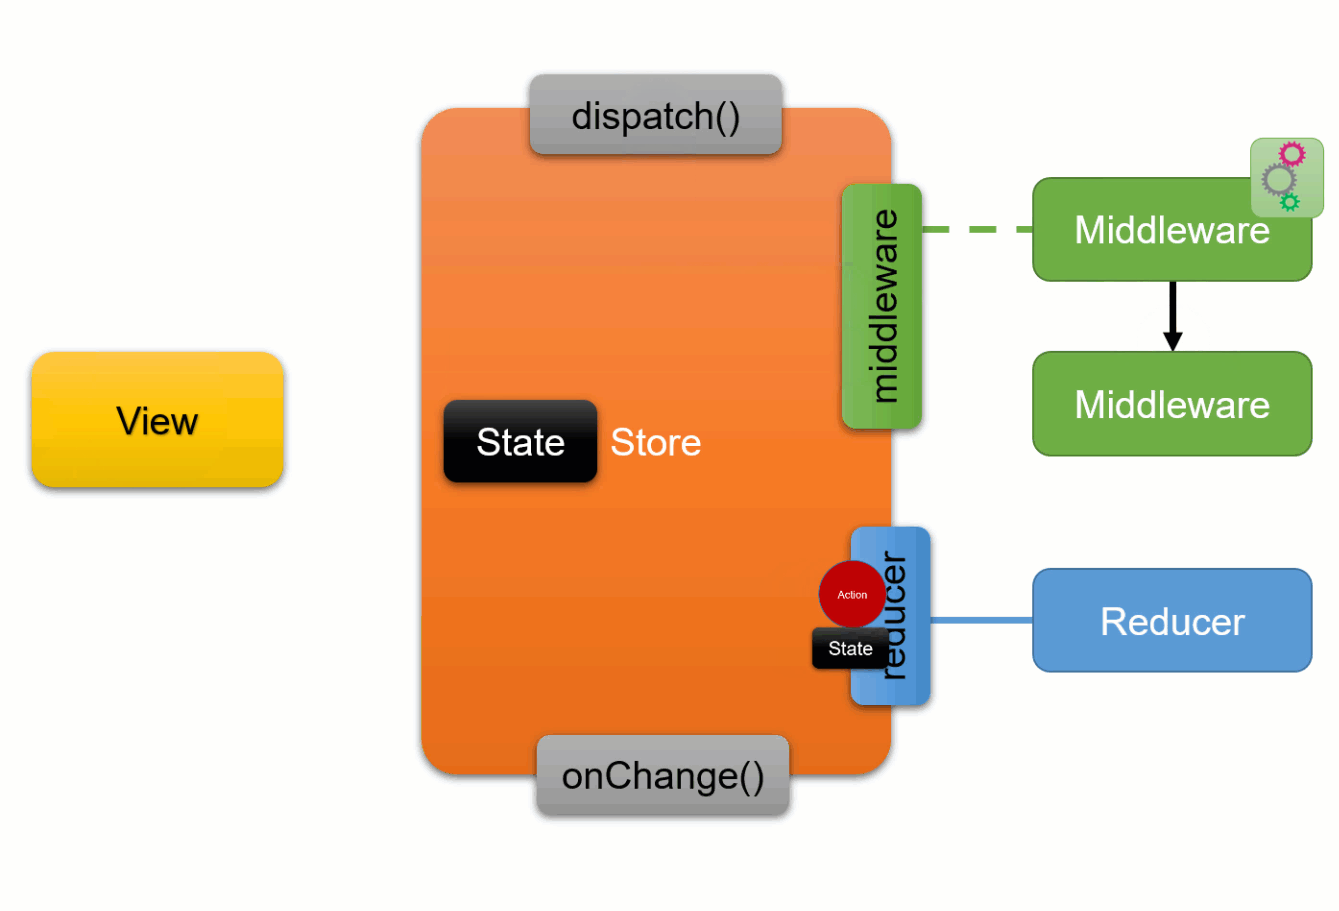
\includegraphics[width=\figureWidthModifier\linewidth]{img/stand-van-zaken/redux-working-detailed-3.png}
    \caption{De Action en de State worden doorgestuurd de Reducer \autocite{Boelens2019}}
    \label{fig:redux-working-detailed-3}
\end{figure}

\begin{figure}[H]
    \centering
    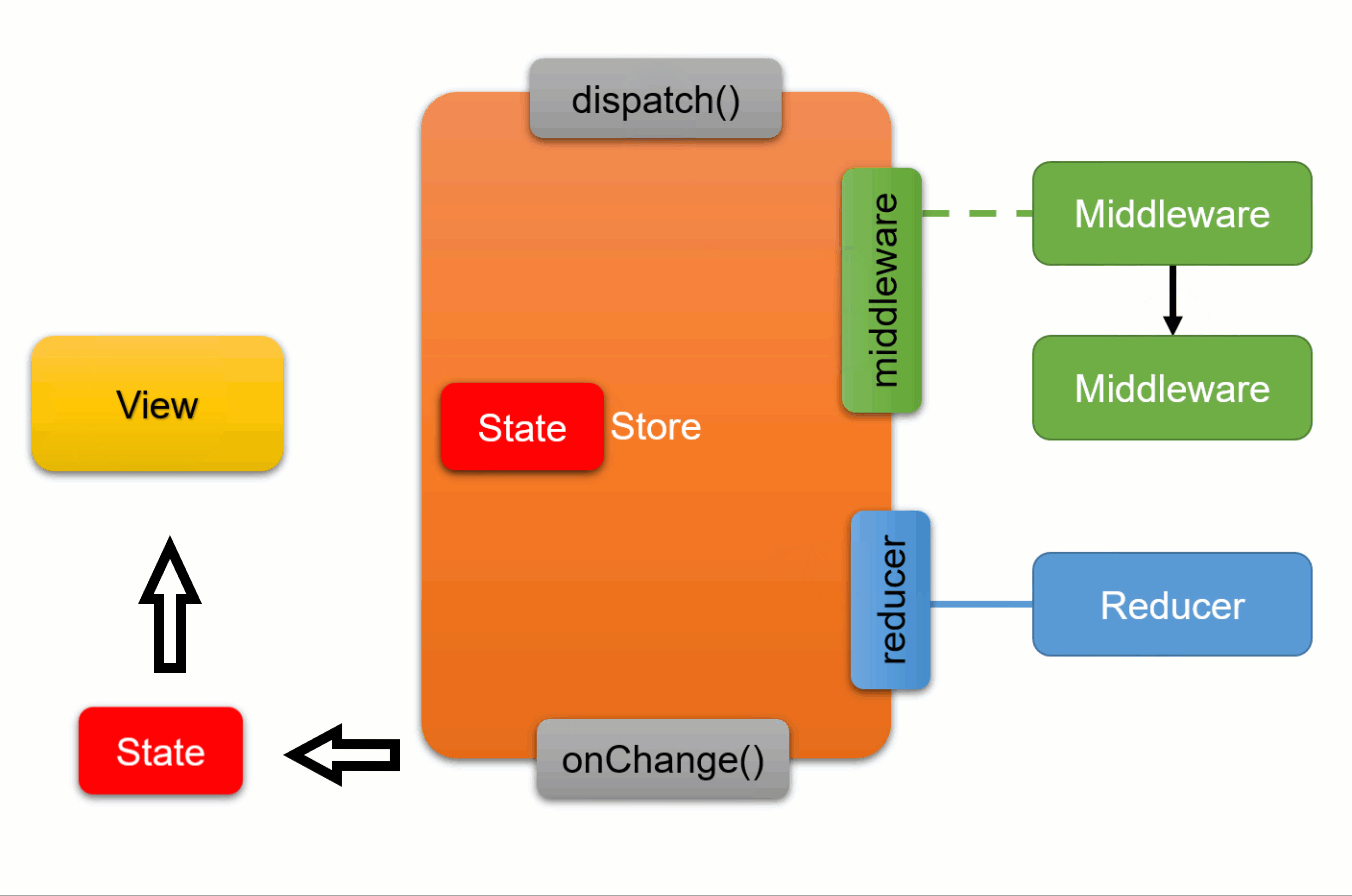
\includegraphics[width=\figureWidthModifier\linewidth]{img/stand-van-zaken/redux-working-detailed-4.png}
    \caption{De view wordt aangepast op basis van de nieuwe State \autocite{Boelens2019}}
    \label{fig:redux-working-detailed-4}
\end{figure}

In het \verb|flutter_redux| package zijn handige widgets beschikbaar. Zo zorgt de \verb|StoreProvider| widget ervoor dat de Redux Store wordt doorgegeven aan alle onderliggende widgets in de widget tree. De \verb|StoreBuilder| haalt de Store uit de \verb|StoreProvider| en geeft die door aan een widget builder function. Het nadeel bij de \verb|StoreBuilder| is dat de widget in de build functie telkens zal worden opnieuw opgebouwd wanneer de State wijzigt, dit kan leiden tot onnodige rerenders. De \verb|StoreConnector| biedt hiervoor de oplossing. De \verb|StoreConnector| haalt de Store uit de dichtstbijzijnde StoreProvider voorouder en zet de Store om in een ViewModel. Dit ViewModel zal alleen de waarde bevatten die van belang is voor desbetreffende widget. Zo wordt een widget niet onnodig opgebouwd wanneer de Store wijzigt, maar alleen wanneer de waarde, gespecifieerd in de ViewModel, wijzigt. Bijvoorbeeld: de Redux Store bevat een counter waarde en een willekeurige tekst, de code voor de StoreConnecter wordt de volgende: 

\begin{minted}{dart}
new StoreConnector<int, CounterViewModel>(
    converter: (store) => CounterViewModel.from(store),
    builder: (context, counterViewModel) {
        return Text(counterViewModel.value);
    },
);
\end{minted}
Hier zal de Text widget alleen heropgebouwd worden wanneer de waardes die relevant zijn voor het CounterViewModel wijzigen.


\subsection{MobX}
\label{ch:mobx}
\subsubsection{Principes}
MobX is opnieuw een library die bekend is bij ontwikkelaars. MobX is beschikbaar in Flutter via de package \verb|mobx|. MobX is een State Management bibliotheek om de gegevens van de applicatie op een simpele manier te verbinden met de UI. Deze verbinding gebeurt volledig automatisch. De ontwikkelaar focust zich enkel op de data die in de UI getoond moet worden zonder zich zorgen te maken over het feit dat deze in sync moeten staan.

MobX maakt gebruikt van drie belangrijke concepten: \textbf{Observables}, \textbf{Actions} en \textbf{Reactions}.
\newline
De Observables bevatten de state van de applicatie. Een Observable kan een primitief datatype zijn tot een zelf geschreven klasse. Met de volgende lijn code wordt een Observable geïnstantieerd. \verb|final counter = Observable(0);|.

De Actions definiëren hoe de Observables gemuteerd moeten worden. Opnieuw is, zoals in Redux, een scheiding gemaakt zodat de waarden nooit direct aangepast kunnen worden.
Een voorbeeld van een Action:
\begin{minted}{dart}
final increment = Action((){
    counter.value++;
});    
\end{minted}

De Reactions voltooien de MobX-triade. De Reactions zijn de waarnemers van de Observables. Een Reaction houdt als het ware een Observable bij. Telkens wanneer een Observable wijzigt, wordt de Reaction verwittigd. Er zijn een paar verschillende vormen van een Reaction, maar deze geven allemaal een \verb|ReactionDisposer| terug. Deze \verb|ReactionDisposer| is een functie dat kan wordt opgeroepen om de reaction weg te verwijderen uit het geheugen. Een voorbeeld van de \verb|autorun| Reaction:
\begin{minted}{dart}
int counter = Observable(0);

final dispose = autorun((_) {
    print(counter);
});

counter = 1;

dispose();

// Prints:
// 0
// 1
\end{minted}

Deze drie principes zijn terug te vinden op figuur \ref{fig:mobx-principles}:

\begin{figure}[H]
    \centering
    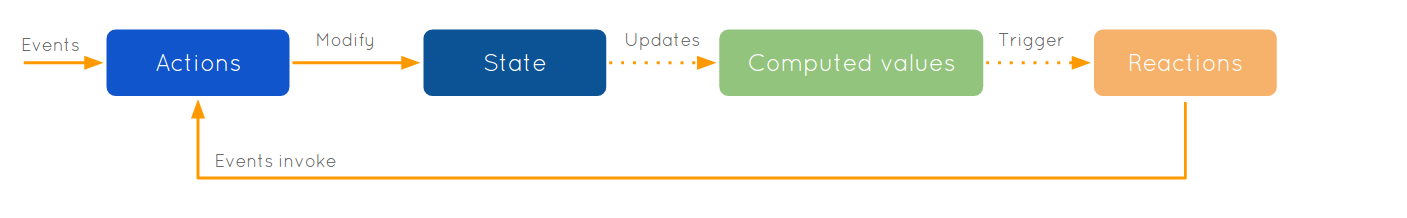
\includegraphics[width=\linewidth]{img/stand-van-zaken/mobx-principles.png}
    \caption{Flowchart van MobX \autocite{MobX2019}}
    \label{fig:mobx-principles}
\end{figure}

Een ander begrip dat terug komt in MobX is een Store. Dit is een klasse die de bijhorende Observables zal bevatten. Bijvoorbeeld een counter Store zal de waarde bijhouden van de counter inclusief een actie om deze te incrementeren.

De  \verb|flutter_mobx| package bevat tal van handige widgets zoals een Observer widget die automatisch wordt opgebouwd wanneer de waarde van een Observable wijzigt. 
Om de Store klasse leesbaar te houden wordt gebruikt gemaakt van \verb|mobx_codegen|. Deze package zorgt dat er geen boilerplate code geschreven moet worden. 

%%=============================================================================
%% Methodologie
%%=============================================================================

\chapter{\IfLanguageName{dutch}{Methodologie}{Methodology}}
\label{ch:methodologie}

\section{Inleiding}
Om een antwoord te krijgen op de onderzoeksvraag wordt een experiment opgesteld. In dit experiment wordt een mobiele applicatie ontwikkeld voor de reeds opgesomde benaderingen van State Management. Dit experiment zal, per benadering van de verschillende State Management, twee resultaten opleveren. Het eerste resultaat zal het aantal lijnen code van het project bevatten per benadering. Hoe deze meting te werk zal gaan wordt in sectie \ref{ch:loc} besproken. Als tweede resultaat wordt een automatische procedure een aantal keer doorlopen, dit wordt uitvoerig besproken in sectie \ref{ch:prestaties}. \newline
Als eerst worden de nodige voorbereidingen voor dit experiment besproken.

\section{Voorbereidingen}
\subsection{De applicatie}
De applicatie heet ``Store It'. Het hoofddoel van de applicatie is om producten te bekijken en toe te voegen. De koper heeft als doel de lijst van producten te raadplegen. Alsook de details van een product te bekijken en eventueel een product te verwijderen. Een verkoper heeft als hoofddoel om een product toe te voegen. Om de complexiteit van de applicatie te beperken wordt geen onderscheid gemaakt tussen een klant en een verkoper.\newline

De layout van de mobiele applicatie is gebasseerd op mock-ups, zie figuren \ref{fig:mock-ups-store-it}. Deze mock-ups werden op voorhand gemaakt zodat tijdens het ontwikkelen van de applicatie geen tijd besteed wordt aan de visuele aspecten.

\begin{figure}
    \begin{tabular}{cc}
        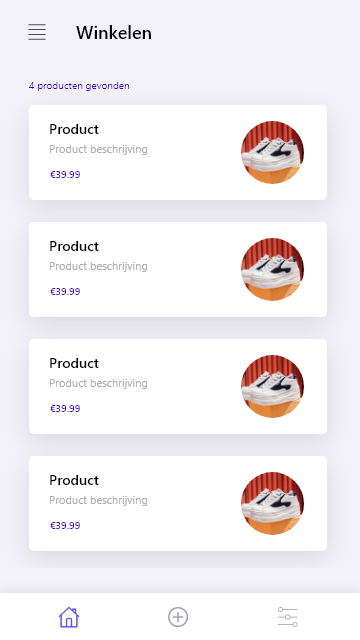
\includegraphics[width=65mm]{img/methodologie/mock-home_screen.png} &   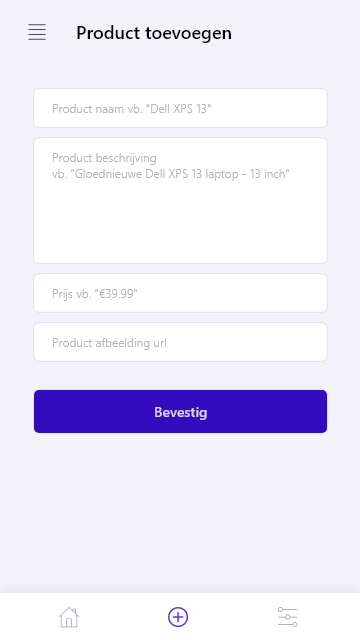
\includegraphics[width=65mm]{img/methodologie/mock-add_product_screen.png} \\
        (a) Mock-up: product lijst pagina & (b) Mock-up: product toevoegen pagina\\[6pt]
        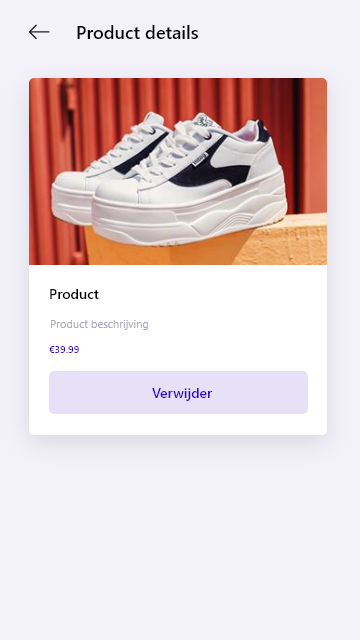
\includegraphics[width=65mm]{img/methodologie/mock-details_screen.png} &   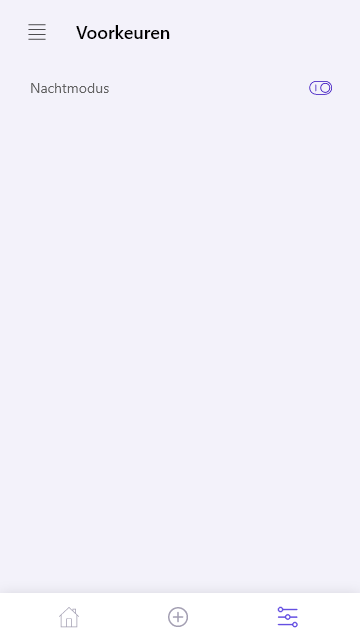
\includegraphics[width=65mm]{img/methodologie/mock-preferences.png} \\
        (c) Mock-up: product details pagina & (d) Mock-up: Voorkeuren pagina \\[6pt]
    \end{tabular}
    \caption{Mock-ups van Store It}
    \label{fig:mock-ups-store-it}
\end{figure}

\subsubsection{Schermen}
De Store It applicatie bestaat uit vier schermen: 
\begin{itemize}
    \item De ``start'' pagina met een lijst van de producten
    \item De ``voeg-product-toe'' pagina met een formulier om een product toe te voegen
    \item De ``voorkeuren'' pagina met een mogelijkheid om het thema van de applicatie te wijzigen
    \item De ``details'' pagina met de details van een geselecteerd product
\end{itemize}

De Store It applicatie maakt het navigeren mogelijk met een \verb|BottomNavigationBar|. De applicatie start op de startpagina, waar de lijst met beschikbare producten wordt weergegeven. Om de geselecteerde tab van de bottom navigation bar bij te houden, wordt gebruikt gemaakt van een index. Deze index wijzigt wanneer een gebruiker op een item in de bottom navigation bar klikt. Om de state bij te werken voor het wijzigen van de index wordt gebruik gemaakt van \verb|setState()|. De index van de startpagina, voeg-product-toe pagina en voorkeuren pagina zijn respectievelijk 0, 1, 2.
Op basis van deze index wordt de bijhorende pagina getoond.

Wanneer een gebruiker op een product klikt, wordt de detailspagina geopend. \newline
De gebruiker heeft de mogelijkheid om het product te verwijderen op de detailspagina. Indien het product is verwijderd, wordt een snackbar getoond met een bevestiging en wordt de gebruik herleid naar de startpagina.
De detailspagina is de enige pagina die bovenop de actieve pagina wordt gepusht. Deze pagina beschikt over een terug knop die de detailspagina zal ``poppen''.

Op de voeg-product-toe pagina wordt een invulformulier getoond. Hier kan de gebruiker een nieuw product toevoegen. De invoervelden beschikken over standaard validatie waarbij de ingevoerde waarde niet leeg mag zijn. Indien deze validatie niet is voldaan, wordt een gepaste melding onder desbetreffend invoerveld getoond. \newline
Wanneer de gebruiker bevestigt, wordt het product toegevoegd aan de lijst op de startpagina. Merk op dat op dit moment deze productlijst niet getoond wordt aangezien de gebruiker zich op de voeg-product-toe pagina bevindt.

Op de voorkeurenpagina kan de gebruiker het thema aanpassen, dit gebeurt met de \verb|Switch| widget. Standaard start de applicatie in een licht thema. De gebruiker kan naarmate zijn/haar voorkeuren het thema aanpassen. De mogelijke thema's zijn licht en donker.
Wanneer het thema wijzigt, wordt de gehele applicatie aangepast naar het geselecteerde thema. Aangezien de gehele applicatie moet gewijzigd worden, is dit een interessante pagina op vlak van state. Namelijk elk widget in de widget tree moet opnieuw gebouwd worden om de wijzigingen ``at runtime'' toe te passen.


De broncode is beschikbaar op \url{https://github.com/devrnt/bachelor-thesis-store-it} \autocite{DeVrient2019}. De \verb|master| tak bevat de boilerplate code. De verschillende benaderingen zijn onderveeld per tak. Zo bevat de \verb|mobx| tak de MobX State Management benadering.

\section{Aantal lijnen code}
\label{ch:loc}
Om een benaderend meetniveau te verkrijgen voor de complexiteit van een State Management worden de aantal lijnen code geteld. Dit resultaat zal een beeld scheppen op de hoeveelheid code die geschreven moet worden om een benadering van State Management uit te schrijven. Merk op dat de complexiteit van een benadering verschillend is van ontwikkelaar tot ontwikkelaar, dit is en blijft een subjectief meetniveau. Uit dit resultaat wordt besloten hoe vlot een benadering van State Management geschreven kan worden.  

De aantal lijnen code van de Dart bestanden worden geteld. De Dart bestanden worden gekenmerkt door de \verb|.dart| extensie. Hiervoor wordt per verschillende benadering het volgende commando gebruikt: \verb=find ./lib/ -name '*.dart' \| xargs wc -l=. Dit commando geeft het totaal aantal lijnen code terug, dit zal per verschillende benadering uitgevoerd worden. \newline 
Tijdens het schrijven van de benaderingen wordt er rekening gehouden met volgende afspraken: commentaar in de code wordt, voor het commando wordt uitgevoerd, verwijderd. Er wordt enkel gebruik gemaakt van een backspace (nieuwe lijn) voor de scheiding van de verschillende methodes. Deze afspraken worden strict nagestreefd doorheen de verschillende benaderingen. \newline
\newline
Vooraleer de aantal lijnen code worden geteld, wordt de broncode van de verschillende benaderingen geformateerd. In dit experiment wordt de \verb|dart_style| package gebruikt als formatter. Deze formatter hanteert de richtlijnen van de Dart style guide \autocite{Dart2019a}. De \verb|line-length| wordt ingesteld op 90. Dit houdt in, dat lijnen die langer zijn dan 90 karakters, gebroken worden en op een nieuwe lijn verder lopen. Om de code te formatteren wordt volgend commando uitgevoerd: \verb|flutter format -l 90 ./lib/|.


\section{Prestaties}
\label{ch:prestaties}
\subsection{Integratietesten}
Flutter beschikt over de nodige tools voor het uitvoeren van integratietesten. Deze testen schrijven de gebruikersflow uit, waardoor individuele modules als één geheel getest kunnen worden. Tijdens een integratie test wordt een gebruikersflow uitgeschreven en vervolgens gesimuleerd op een apparaat \autocite{Flutter2019b}. 

Een integratie test bestaat uit de eindapplicatie, die ook gebruikt zou worden in productie, en een test suite. De test suite definieert de stappen die doorlopen worden tijdens de integratie test. Een voorbeeld van een flow: \textit{De gebruiker klikt op een product, vervolgens verwijdert de gebruiker het product...}. Zie \ref{ch:user-flow} gebruikersflow voor dit experiment. De test suite vindt de nodige widgets in de applicatie door een unieke \verb|key| te definiëren in de broncode. In de test suite wordt het widget opgeroepen met: \verb|find.byValueKey('product-item')|. \newline
Deze integratietesten worden in dit experiment gebruikt om de automatische gebruiker-flow uit te schrijven. Zodanig dat telkens hetzelfde pad wordt doorlopen per benadering van State Management.

Om de effectieve integratietesten te schrijven wordt de \verb|flutter_driver| package gebruikt.
Een integratie test maakt een instrumentale versie van de applicatie. Deze instrumentale versie maakt het mogelijk om de applicatie te besturen (met de stappen uit de test suite) en prestaties te capteren.
De integratietesten worden uitgevoerd in de profile modus van Flutter. De profile modus compileert en start een applicatie bijna identiek als de release mode (productie) en beschikt over de extra functionaliteit om prestatieproblemen te capteren en te debuggen.

\subsection{Gebruikersflow}
\label{ch:user-flow}
In dit experiment ligt de focus van de verschillende benaderingen van State Management op volgende zaken: 
\begin{itemize}
    \item De gebruiker wijzigt het thema op de voorkeurenpagina.
    \item De gebruiker voegt een nieuw product toe, als gevolg dat de lijst van producten moet bijgewerkt worden op de andere pagina.
    \item De gebruiker verwijdert een product op het detailspagina, als gevolg dat de lijst van producten moet bijgewerkt worden op de startpagina.
\end{itemize}
Voor deze opsomming zal per benadering de broncode worden aangepast. De broncode van een benadering van een State Management wordt gestart vanaf boilerplate code. Deze boilerplate code werd op voorhand geschreven. Deze code bevat onder andere de gemeenschappelijke widgets, bijvoorbeeld een product-item, de knoppen...
Bij deze template is geen sprake van State Management, buiten de state van de \verb|BottomNavigationBar|. De rest van de state wordt aangevuld per verschillende benadering.

De test suite bevat de volgende stappen die chronologisch worden uitgevoerd:
\begin{enumerate}
    \item De gebruiker opent de applicatie en navigeert naar de startpagina
    \item De gebruiker klikt op het laatste product in de lijst
    \item De gebruiker verwijdert het product
    \item De gebruiker navigeert naar de startpagina
    \item De gebruiker navigeert naar de voeg-product-toe pagina
    \item De gebruiker vult het formulier in en voegt het product toe
    \item De gebruiker navigeert naar de startpagina
    \item De gebruiker klikt op het nieuwe product
    \item De gebruiker verwijdert het nieuwe product
    \item De gebruiker navigeert naar het voorkeurenpagina
    \item De gebruiker klikt op de nachtmodus switch
    \item De gebruiker navigeert naar de startpagina
    \item De gebruiker klikt op een product
    \item De gebruiker verwijdert het product
    \item De gebruiker navigeert naar de voeg-product-toe pagina
    \item De gebruiker vult het formulier in en voegt het product toe
    \item De gebruiker navigeert naar de startpagina
    \item De gebruiker sluit de applicatie
\end{enumerate}

De uitvoering van deze stappen zijn te zien in de video. \autocite{DeVrient2019f}

Tijdens het doorlopen van de stappen wordt data gecapteerd. Deze data wordt in Flutter beschouwd als een \verb|Timeline| object. Het \verb|Timeline| object bevat de ruwe uitvoer van de uitgevoerde stappen. Dit JSON-bestand kan bekeken worden in Google Chrome via \verb|chrome://tracing| en resulteert in een visuele voorstelling van de data, te zien op figuur \ref{fig:chrome-tracing-timeline}. Deze uitvoer bevat tal van gemeten waarden. De CPU-tijd is samen met de overgeslagen frames voor dit onderzoek de belangrijkste, gemeten data. 

De stappen worden per benadering doorlopen. Deze procedure zal voor elke benadering 50 keer uitgevoerd worden. Dit zorgt voor voldoende resultaten om te analyseren. Zo wordt ook, de kans dat een conclusie wordt gebasseerd op toevallige meetresulaten, verkleind.

\begin{figure}[H]
    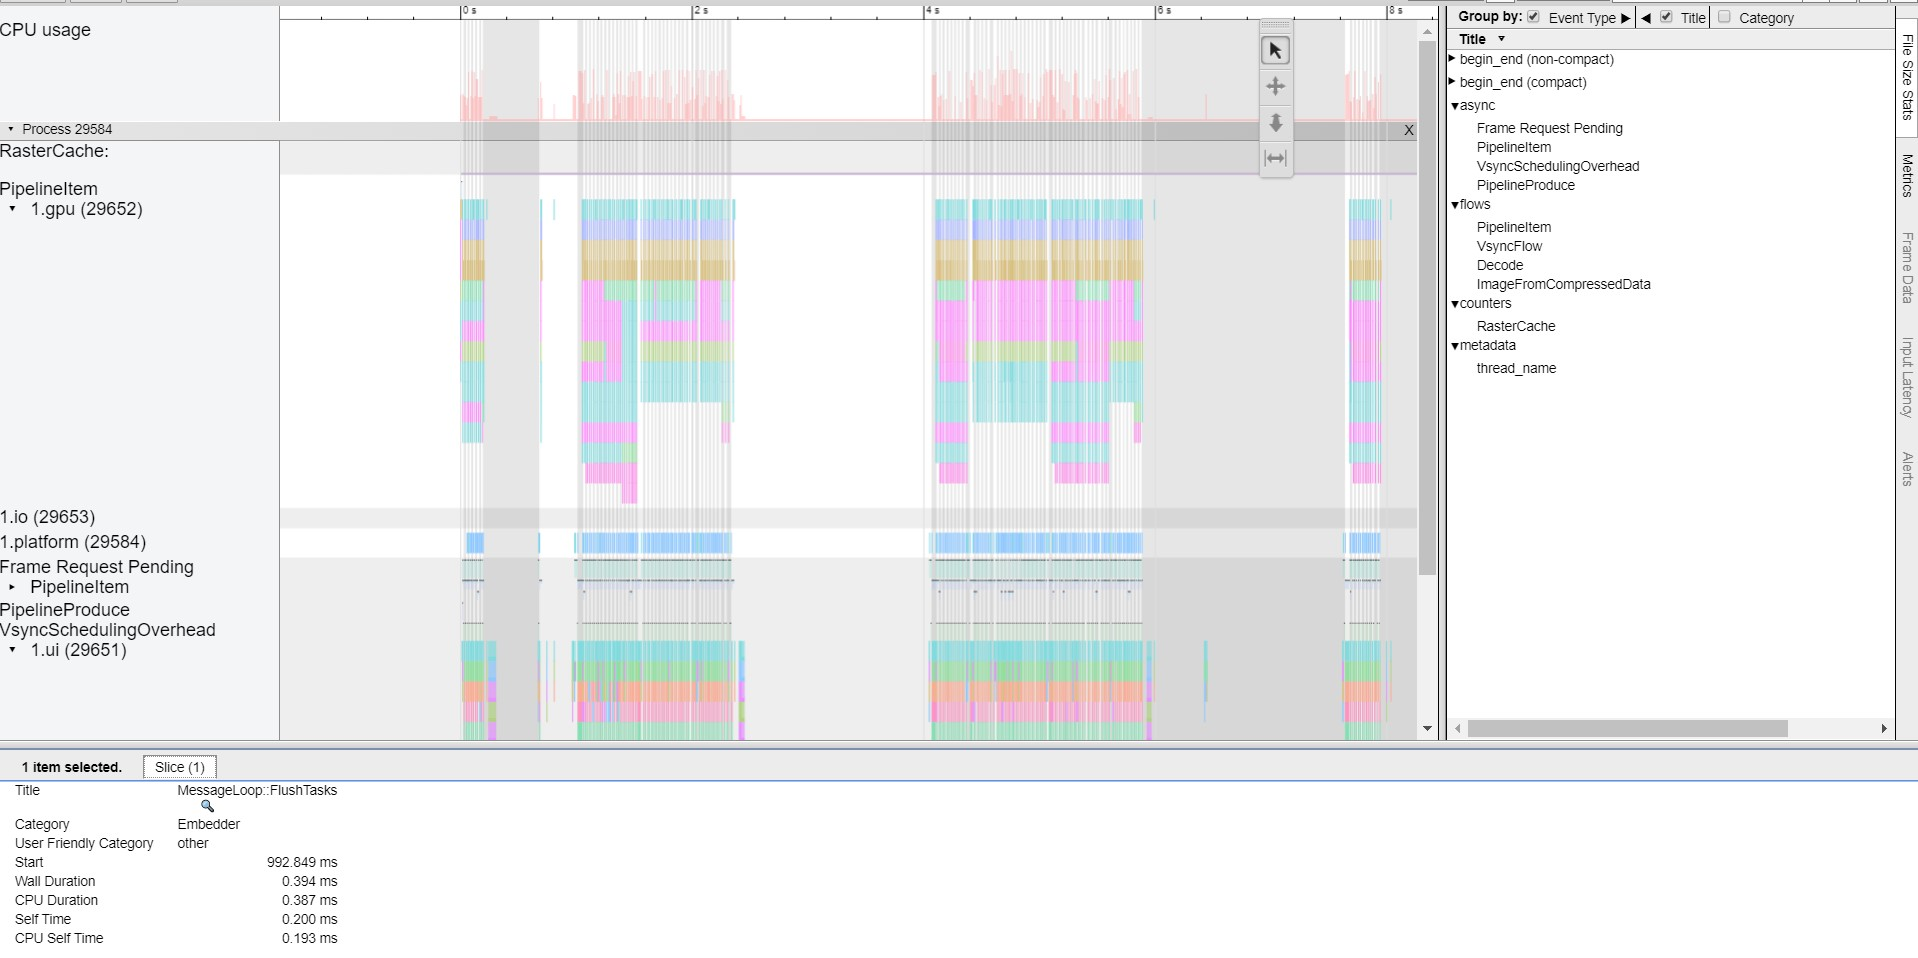
\includegraphics[width=\linewidth]{img/methodologie/chrome-tracing-timeline.jpg}
    \caption{Visuele voorstelling van de ruwe uitvoer in chrome://tracing}
    \label{fig:chrome-tracing-timeline}
\end{figure}


\subsection{Test apparaat}
Hoewel een iOS Simulator en een Android Emulator goed van pas komen tijdens de ontwikkeling van een applicatie wordt voor het meten van de resultaten beroep gedaan op een fysiek apparaat. De meetresultaten die verkregen zouden worden op een emulator zullen verre van een realistische reflectie zijn op de verkregen resultaten op een fysiek apparaat. \autocite{Flutter2019c}

Flutter laat het ook niet toe om de profile modus uit te voeren op een emulator.
Het test apparaat is een OnePlus 3T, zie tabel \ref{table:specifications-test-device} voor de specificaties.
Nadat de broncode voor elke State Management benadering en integratietesten geschreven zijn, kunnen de resulaten verworven worden voor het experiment.

Samengevat worden voor elke bendaring de gegeven stappen doorlopen door middel van de Flutter integration tests. Tijdens deze procedure wordt de verworven data weggeschreven in een bestand. Dit bestand bevat de nodige meetstaven om verder te gaan met de analyse van de resulaten.

\begin{table}[H]
    \centering
    \begin{tabular}{ll}
        Model & A3003 \\
        Besturingssysteem & Android 9.0 - OxygenOS 9.0.6 \\
        Chipset & Qualcomm MSM8996 Snapdragon 821 (14 nm)  \\
        CPU & Quad-core (2x2.35 GHz Kryo \& 2x1.6 GHz Kryo) \\
        GPU &  Adreno 530 \\
        Geheugen & 6GB RAM \\
        Opslag & 64GB \\ 
        &
    \end{tabular}
    \caption{Specificaties van het test apparaat}
    \label{table:specifications-test-device}
\end{table}



% Voeg hier je eigen hoofdstukken toe die de ``corpus'' van je bachelorproef
% vormen. De structuur en titels hangen af van je eigen onderzoek. Je kan bv.
% elke fase in je onderzoek in een apart hoofdstuk bespreken.

%\input{...}
%\input{...}
%...

%%=============================================================================
%% Conclusie
%%=============================================================================

\chapter{Conclusie}
\label{ch:conclusie}

% Trek een duidelijke conclusie, in de vorm van een antwoord op de
% onderzoeksvra(a)g(en). Wat was jouw bijdrage aan het onderzoeksdomein en
% hoe biedt dit meerwaarde aan het vakgebied/doelgroep? 
% Reflecteer kritisch over het resultaat. In Engelse teksten wordt deze sectie
% ``Discussion'' genoemd. Had je deze uitkomst verwacht? Zijn er zaken die nog
% niet duidelijk zijn?
% Heeft het onderzoek geleid tot nieuwe vragen die uitnodigen tot verder 
%onderzoek?

\section{Antwoord op de onderzoeksvragen}
\subsubsection{Hoeveel verschilt de geschreven code bij verschillende benaderingen van State Management, met andere woorden hoe snel kan een benadering van State Management geschreven worden?}
De ScopedModel en Provider benadering hebben met voorsprong de minst aantal lijnen code. Redux heeft overduidelijk het meest aantal lijnen code. Dit valt te verklaren door de hoeveelheid repetitieve code die geschreven moet worden. 

De benaderingen die het snelst zijn uit te schrijven zijn ScopedModel en Provider. Als nieuwkomer bij het Flutter framework is het aan te raden om gebruik te maken van deze benaderingen. Deze benaderingen vereisen niet alleen weinig code, ze zijn ook instapklaar zonder veel inwerking.  

De Redux benadering valt niet aan te raden voor een Flutter nieuwkomer vanwege de hoeveelheid code die geschreven moet worden. De Redux benadering vereist ook de nodige inwerkingstijd. De ontwikkelaar moet eerst ingewerkt zijn in het Redux ecosysteem vooraleer deze kan gebruikt worden als oplossing voor State Management. 

Hetzelfde geldt voor de MobX en BLoC benadering maar in mindere mate. Deze benaderingen vergen ook een bepaalde inwerkingsperiode, maar zijn minder complex dan Redux. De MobX en BLoC benaderingen zijn sneller uit te schrijven dan Redux benadering, maar minder snel dan de ScopedModel en Provider benadering.

\subsubsection{Hoe variëren de prestaties bij de verschillende benaderingen van State Management?}

Uit dit onderzoek blijk dat de Provider State Management benadering resulteert in de beste performantie. Deze conclusie is gebaseerd op de CPU-tijden en overgeslagen frames, deze resultaten zijn terug te vinden in tabel \ref{table:experiment-cpu-time-conclusion} en in tabel \ref{table:experiment-skipped-frames-conclusion}. Hieruit kan echter niet geconcludeerd worden dat Provider altijd de beste benadering zal zijn. \newline \newline
Als eerst is de applicatie in dit experiment geen volledige voorstelling van een applicatie in de echte wereld. In dit experiment wordt enkel rekening gehouden met state in de applicatie, zonder data op te halen van een externe backend. In deze applicatie worden de producten niet opgehaald door middel van een netwerk verzoek, er wordt enkel gebruik gemaakt van gemockte producten. Dit experiment representatief voor applicaties die enkel gebruik maakt van lokale state. Het moet verder worden onderzocht of de getrokken conclusies gelden voor een applicatie die netwerk verzoeken stuurt. \newline
Het is perfect mogelijk om de netwerk verzoeken te integreren in de State Management van deze applicatie. Dit zal voor enkele benaderingen meer werk vergen dan voor andere. Zo zullen de netwerk verzoeken relatief snel geïntegreerd kunnen worden in de BLoC benadering aangezien er reeds gebruikt gemaakt wordt van asynchronous stream. \newline 

\begin{table}[H]
    \centering
    \begin{tabular}{c|c|c|c|c|c}
        & \textbf{ScopedModel} & \textbf{Provider} & \textbf{BLoC} & \textbf{Redux} & \textbf{MobX} \\ \hline
        Minimum             & 4026.77    & 2904.56    &  3495.19   &  3727.69  &  3950.13      \\ \hline
        Maximum             & 6595.28    & 5486.11    &  5529.18   &  6546.53  &  5655.71      \\ \hline
        Gemiddelde          & 5838.15    & 4741.56    &  4884.95   &  5512.45  &  4849.02      \\ \hline
        Mediaan             & 5908.59    & 4869.92    &  4946.48   &  5601.20  &  4905.71      \\ \hline
        Standaardafwijking  & 492.11     & 485.12     &  393.12    &  625      &  358.07       \\ \hline
        Variantie           & 242174.60  & 235343.70  &  154543    &  390629   &  128216.90    \\ \hline
        Modus               & 6029.70    & 4576.04    &  5061.23   &  4597.65  &  4915.30      \\                
    \end{tabular}
    \caption{Statistieken van de CPU-tijd (in ms) van alle benaderningen}
    \label{table:experiment-cpu-time-conclusion}
\end{table}

\begin{table}[H]
    \centering
    \begin{tabular}{c|c|c|c|c|c}
        & \textbf{ScopedModel} & \textbf{Provider} & \textbf{BLoC} & \textbf{Redux} & \textbf{MobX} \\ \hline
        Totaal      &  838   &  595     &  610     &  820    &  572        \\ \hline
        Gemiddeld   &  16.76    &  11.90   &  12.20   &  16.73  &  11.40        \\ 
    \end{tabular}
    \caption{Statistieken van de totaal en gemiddeld aantal overgeslagen frames van alle benaderingen}
    \label{table:experiment-skipped-frames-conclusion}
\end{table}

Als tweede houdt dit experiment enkel rekening met de CPU-tijd en de overgeslagen frames. De data die verworven is tijdens het doorlopen van de verschillende benaderingen bevat tal van andere maatstaven. Uit deze data werd voor dit onderzoek enkel en alleen gekeken naar de CPU-tijd en de overgeslagen frames, maar het is perfect mogelijk om rekening te houden met meer maatstaven. Zo is het mogelijk om rekening te houden met de build times en de rasterzation times. Rasterisation is het concept waarbij een beeld dat bestaat uit vormen wordt omgezet naar een reeks van pixels om zo het gewenste beeld te bekomen. \newline \newline
Als derde opmerking: tijdens het doorlopen van de verschillende benaderingen op het test apparaat werd dit uitgevoerd op een Android toestel. Dit testapparaat behoort heden tot de mid-range smartphones. Er zou getest kunnen worden of gelijkaardige resultaten bekomen worden bij het uitvoeren van dezelfde gebruikersflow bij andere segmenten van de smartphones. Onder andere op een smartphone met mindere specificaties alsook een met hogere specificaties. Het kan bijvoorbeeld zijn dat de Redux benadering die slecht scoort op het testapparaat van dit experiment het beter doet op een apparaat met betere specificaties. 

Als laatste werd dit experiment de gebruikersflow enkel doorlopen op een Android toestel. Het zou interessant zijn om dezelfde gebruikersflow uit te voeren op een iOS testappraat. 

De CPU-tijd van een applicatie is slechts één indicator om de performantie ervan aan te tonen.

\section{Conclusie van deze bachelorproef}
In het begin van dit onderzoek werd de hoofdonderzoeksvraag gegeven en die luidde als volgt: \textit{Hoeveel impact hebben verschillende benaderingen van State Management in Flutter?} Om dit te onderzoeken werd een keuze gemaakt aan bepaalde meetcriteria, aangezien impact een overkoepelende term is. Zo werd rekening gehouden met het aantal lijnen code, de CPU-tijd en de overgeslagen frames. \newline \newline
Uit dit onderzoek kan er vast gesteld worden dat de Provider State Management benadering uitblinkt op vlak van het aantal lijnen code, de CPU-tijd en aantal overgeslagen frames. \newline
De ontwikkelaar kiest nog steeds zijn/haar voorkeur voor welke benadering toe te passen. \newline \newline
Deze bachelorproef loopt hier zeker niet ten einde, het biedt tal van uitbreidingsmogelijkheden. Zo kan hetzelfde onderzoek uitgevoerd worden op een iOS apparaat en kan rekening gehouden worden met extra meetstaven, zoals de build times en de rasterization times.

%%=============================================================================
%% Bijlagen
%%=============================================================================

\appendix
\renewcommand{\chaptername}{Appendix}

%%---------- Onderzoeksvoorstel -----------------------------------------------

\chapter{Onderzoeksvoorstel}

Het onderwerp van deze bachelorproef is gebaseerd op een onderzoeksvoorstel dat vooraf werd beoordeeld door de promotor. Dat voorstel is opgenomen in deze bijlage.

% Verwijzing naar het bestand met de inhoud van het onderzoeksvoorstel
%---------- Inleiding ---------------------------------------------------------

\section{Introductie} % The \section*{} command stops section numbering
\label{sec:introductie}

Flutter de UI-toolkit van Google voor het ontwikkelen van mobiele-, web- en desktop applicaties,
heeft gezorgd voor een opvallende beweging omtrend ontwikkelings frameworks.
Nog geen jaar na de officiële release zijn bedrijven in actie geschoten met het implementeren van Flutter
in hun applicaties.
Met als grootste concurrent React Native heeft Flutter enkele oorzaken voor haar populariteit: snelle ontwikkelingsomgeving (Hot Reload) en native prestaties zijn hier enkele van.
Door de toenemende populariteit is er als maar meer vraag gekomen van zowel beginnende als
reeds ervaren ontwikkelaars naar de ``juiste manier'' voor het benaderen van State Management in Flutter.
State Mangement kan kort omschreven worden als het resultaat van alle acties die de gebruiker heeft
uitgevoerd.
Denk maar aan een incrementeer knop die de waarde van een teller verhoogt wanneer op de knop wordt gedrukt, hier moet de state van de teller bijgehouden worden.

Door het ontwikkelingsteam van Flutter wordt State Management beschouwd als een complex onderwerp. Volgens hen bestaat geen perfecte benadering van State Managementen, een bepaalde benadering zal altijd zijn voor- en nadelen hebben.

Zowel nieuwkomers in het Flutter framework als reeds ervaren ontwikkelaars hebben 
veel onzekerheden over de benadering van State Management.
Het doel van dit onderzoek is om een duidelijk beeld te scheppen over hoeveel impact
verschillende benaderingen van een State Management in Flutter hebben op een applicatie.
Tijdens het onderzoek wordt er gekeken naar de complexiteit van de gekozen benadering van State Management en de gevolgen ervan voor de prestaties.

Met oog op het bekomen van een conclusie voor dit onderzoek
zullen onderstaande onderzoeksvragen eerst beantwoord moeten worden:
\begin{itemize}
    \item Hoe ver staat Flutter anno eind 2019?
    \item Wat is State Management in Flutter?
    \item Hoeveel verschilt de geschreven code bij verschillende benaderingen van State Management, m.a.w. hoe snel 
    ken een benadering van State Management geschreven worden?
    \item Hoe variëren de prestaties bij de verschillende benaderingen van State Management?
\end{itemize}
    
Deze onderzoeksvragen zullen een antwoord bieden op de hoofdonderzoeksvraag: hoeveel impact hebben verschillende benaderingen van State Management in Flutter.

%---------- Stand van zaken ---------------------------------------------------

\section{State-of-the-art}
\label{sec:state-of-the-art}
\subsection*{Flutter}
Flutter is een relatief nieuw framework. Sinds de eerste stabiele release in december 2018 is de populariteit
van Flutter enorm toegenomen. Door het bereiken van het grote publiek duiken tal van vragen op in verband met 
State Management in Flutter. Op dit moment zijn er nog geen wetenschappelijke artikels verschenen in verband met dit topic.
Er is reeds een vergelijkende studie uitgevoerd tussen React Native, een open-source framework voor mobiele applicaties en Flutter \autocite{Wu2018}.

Verder werd een uitgebreide vergelijking gemaakt hoe Flutter zich verhoudt tegenover native Android, native IOS,
React Native en Xamarin Forums \autocite{Coninck2019}.
Hierin wordt Flutter uitvoerig besproken en wordt een experiment opgesteld waar vergeleken wordt hoelang het duurt
om een applicatie te ontwikkelen met dezelfde layout. Tijdens dit experiment werd ook het performantieverschil gemeten bij de verschillende applicaties. 

%Hier beschrijf je de \emph{state-of-the-art} rondom je gekozen onderzoeksdomein. Dit kan bijvoorbeeld een literatuurstudie zijn. Je mag de titel van deze sectie ook aanpassen (literatuurstudie, stand van zaken, enz.). Zijn er al gelijkaardige onderzoeken gevoerd? Wat concluderen ze? Wat is het verschil met jouw onderzoek? Wat is de relevantie met jouw onderzoek?
%
%Verwijs bij elke introductie van een term of bewering over het domein naar de vakliteratuur, bijvoorbeeld Denk zeker goed na welke werken je refereert en waarom.

% Voor literatuurverwijzingen zijn er twee belangrijke commando's:
% \autocite{KEY} => (Auteur, jaartal) Gebruik dit als de naam van de auteur
%   geen onderdeel is van de zin.
% \textcite{KEY} => Auteur (jaartal)  Gebruik dit als de auteursnaam wel een
%   functie heeft in de zin (bv. ``Uit onderzoek door Doll & Hill (1954) bleek
%   ...'')

%Je mag gerust gebruik maken van subsecties in dit onderdeel.

\subsection*{State Management}
Op de officiële site van Flutter wordt een sectie besteed aan State Management.
Met name op welke manieren state management benaderd kan worden, maar er zijn nog geen grote
onderzoeken of bachelorproeven geschreven waarin de verschillende benaderingen uitvoerig worden getest.

De resultaten van dit onderzoek kunnen gebruikt worden om in verdere stadia van Flutter
een geschikte benadering van State Management te bekomen, rekeninghoudend met de complexiteit en prestaties
van de gekozen benadering.


%---------- Methodologie ------------------------------------------------------
\section{Methodologie}
\label{sec:methodologie}
Tijdens dit onderzoek wordt er een experiment opgesteld waar een mobiele applicatie wordt gemaakt 
telkens met een verschillende benadering van State Management. 
Hierop volgt een analyse waar gekeken wordt hoeveel lijnen code vereist zijn voor het uitschrijven van
desbetreffende benadering van State Management. Dit gedeelte omvat ook het bepalen van de complexiteit.
Bij de ontwikkelde applicatie worden per State Management de prestaties gemeten.
De prestaties kunnen omschreven worden als de gespendeerde tijd op de GPU- en CPU-thread.

De verschillende benaderingen van State Management die tijdens het experiment onderzocht zullen worden zijn de volgende: \emph{InheritedWidget \& InheritedModel}, 
\emph{Provider \& Scoped Model}, \emph{Redux}, \emph{BLoC / Rx} en \emph{MobX}.
Deze verschillende benaderingen worden aangeraden op de officiële site van Flutter.

Dit experiment zal een paar tools vereisten zoals Adobe XD om de layout vast te leggen van de applicatie,
daarnaast zal Microsoft Visual Studio Code gebruikt worden om de applicatie te schrijven.
Tijdens het het ontwikkelen van de mobiele applicatie wordt een Android Emulator gebruikt. Voor het meten van de prestaties zal de applicatie op een fysiek apparaat gebruikt worden, deze resultaten zullen gemeten worden via de DevTools plugin van Dart in Visual Studio Code.

Indien tijdens het experiment problemen optreden wordt er geraadpleegd bij Didier Boelens,
een bekende Belgische pionier in de Flutter community, die ook heeft toegestemd in het helpen van deze bachelorproef.

%
%Hier beschrijf je hoe je van plan bent het onderzoek te voeren. Welke onderzoekstechniek ga je toepassen om elk van je onderzoeksvragen te beantwoorden? Gebruik je hiervoor experimenten, vragenlijsten, simulaties? Je beschrijft ook al welke tools je denkt hiervoor te gebruiken of te ontwikkelen.

%---------- Verwachte resultaten ----------------------------------------------
\section{Verwachte resultaten}
\label{sec:verwachte_resultaten}

De applicaties die geschreven worden in de verschillende benaderingen van State Management zullen
geanalyseerd worden op basis van de complexiteit, instapklaarheid, schaalbaardheid en prestaties.
Er wordt verwacht dat de complexere State Management betere prestaties met zich te weeg zal brengen.
Deze prestaties zullen echter niet met het blote oog te zien zijn, maar zullen zich wel in de 
gemeten cijfers reflecteren.

%Hier beschrijf je welke resultaten je verwacht. Als je metingen en simulaties uitvoert, kan je hier al mock-ups maken van de grafieken samen met de verwachte conclusies. Benoem zeker al je assen en de stukken van de grafiek die je gaat gebruiken. Dit zorgt ervoor dat je concreet weet hoe je je data gaat moeten structureren.

%---------- Verwachte conclusies ----------------------------------------------
\section{Verwachte conclusies}
\label{sec:verwachte_conclusies}
Uit dit onderzoek zal blijken dat \emph{Provider} de meest instapklare benadering van state management
zal zijn, zoals reeds aangeraden door het Flutter team.
Daarnaast zal blijken dat benaderingen door \emph{Redux, Mobx, Bloc} minder instapklaar zijn, maar een 
betere schaalbaarheid hebben.
Het verschil in de gemeten prestaties voor de verschillende benaderingen zullen relatief klein zijn, al dan niet significant verschillend.

Welke benadering voor State Management gekozen wordt is nog steeds subjectief, aangezien elke ontwikkelaar een voorkeur heeft. Dit onderzoek zal er voor zorgen
dat bijkomende argumenten kunnen voorgelegd worden om al dan niet een bepaald State Management te hanteren.


%Hier beschrijf je wat je verwacht uit je onderzoek, met de motivatie waarom. Het is \textbf{niet} erg indien uit je onderzoek andere resultaten en conclusies vloeien dan dat je hier beschrijft: het is dan juist interessant om te onderzoeken waarom jouw hypothesen niet overeenkomen met de resultaten.



%%---------- Andere bijlagen --------------------------------------------------
% TODO: Voeg hier eventuele andere bijlagen toe
%\input{...}

%%---------- Referentielijst --------------------------------------------------

\printbibliography[heading=bibintoc]

\end{document}
